\documentclass[10pt]{beamer}

\usetheme[progressbar=frametitle]{metropolis}
\usepackage{appendixnumberbeamer}
\usepackage{smartdiagram}
\usepackage{booktabs}
\usepackage[scale=2]{ccicons}
\usepackage{tabto}
\usepackage{hyperref}
\usepackage{pgfplots}
\usepgfplotslibrary{dateplot}

\usepackage{xspace}
\newcommand{\themename}{\textbf{\textsc{metropolis}}\xspace}

\title{Version control}
\subtitle{(using git)}
%\date{\today}
%\date{}
\author{\textbf{Danny Awty-Carroll}}
\institute{\tiny{\date{\today}}}
\titlegraphic{\hfill
\includegraphics[height=1cm]{Aberystwyth_University_logo}}


\begin{document}

\maketitle


\setbeamertemplate{frame footer}{ }
\begin{frame}{Sections}
This will focus on using git in windows with a UI
\newline

\setbeamertemplate{section in toc}[sections numbered]
\tableofcontents[hideallsubsections]
\end{frame}




\section{Why version control?}


\begin{frame}[fragile]{What is version control}
This is just the management of versions of a document.\\
One document through time.
\begin{columns}[T]
\begin{column}{.5\textwidth}
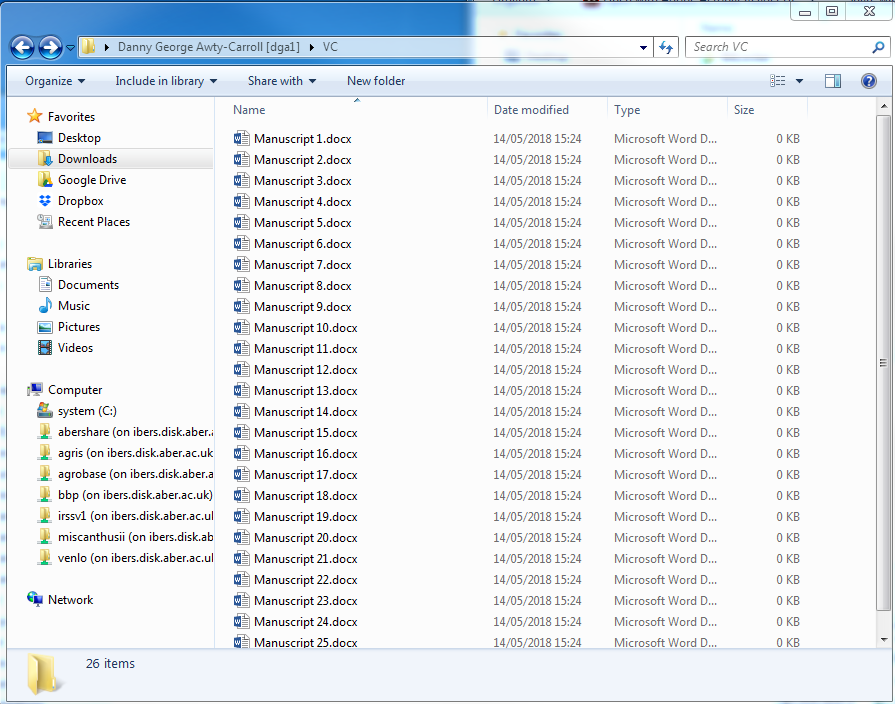
\includegraphics[width=6cm]{Figs/old/no}
\end{column}
\begin{column}{.5\textwidth}
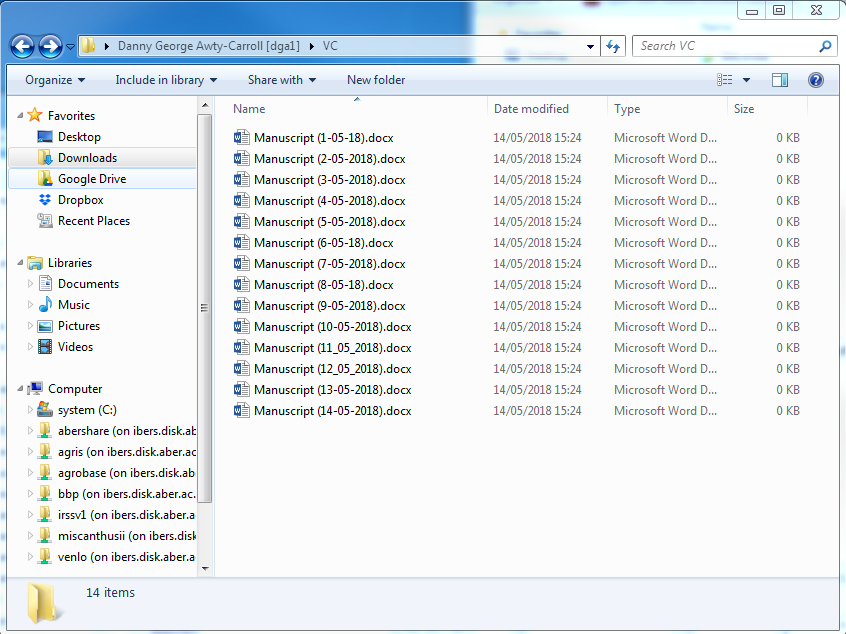
\includegraphics[width=6cm]{Figs/old/date}
\end{column}
\end{columns}
All of us use some version control
\end{frame}


\begin{frame}[fragile]{Where things get complicated}
Numbering or dating documents works OK but can fall down when\\
\begin{itemize}
\item There are multiple documents that need to work together (i.e. a script and data)
\item There are multiple people working on the documents (are they on the latest version and merging changes)
\item There are updates to the project that may break things
\item Line changes need to be reviewed
\end{itemize}

Some of this is solved in programs like word with track changes (so you see who altered what when)
\end{frame}


\begin{frame}[fragile]{What version control systems can do}
\begin{itemize}
\item Give line by line changes linked to a user (which are keeped forever)
\item Makes a stretcher to the version control so there can be side branches (this is where the project can take a detour and be merged back in later)
\item Minimise problems of multiple users working on the same document at the same time
\end{itemize}
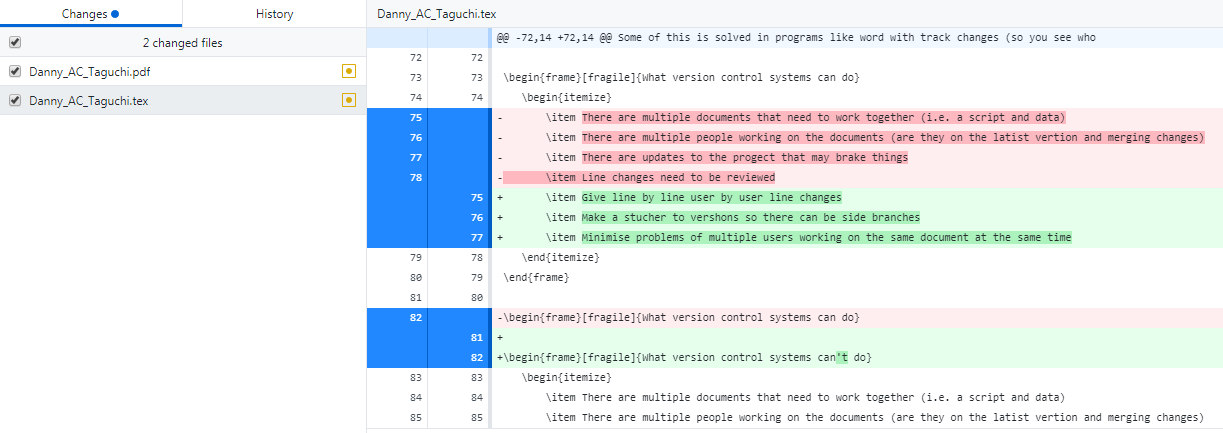
\includegraphics[width=11cm]{Figs/GHD/change}
\end{frame}


\begin{frame}[fragile]{What version control systems can't do}
\begin{itemize}
\item Add much extra control to binary files (not plan text)
\item Back up in real time
\end{itemize}
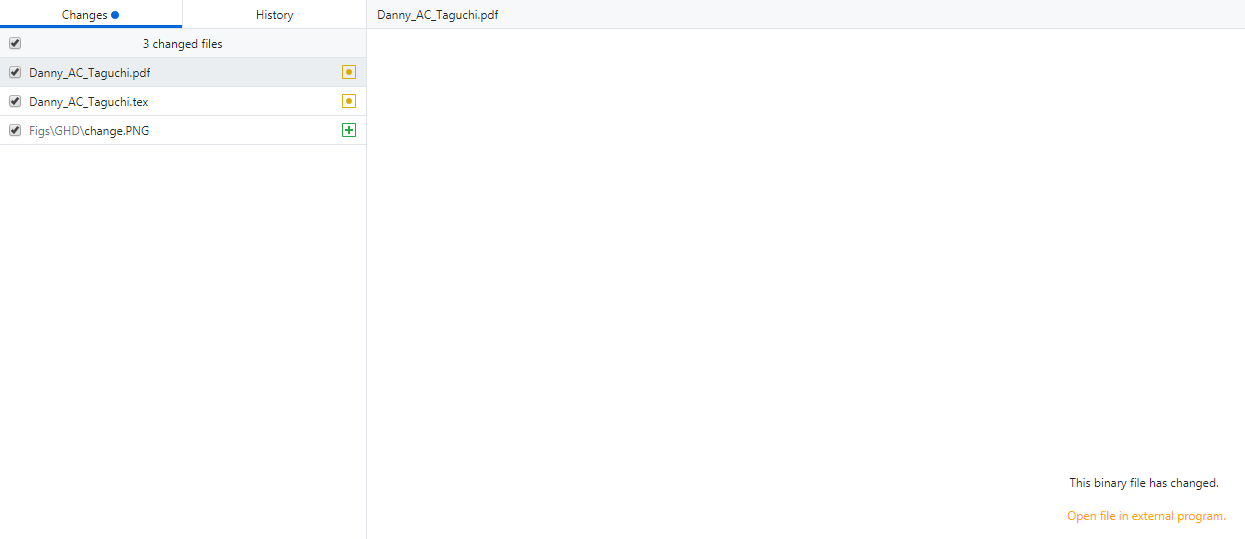
\includegraphics[width=11cm]{Figs/GHD/binarychange}
\end{frame}



\section{Version control system}


\begin{frame}[fragile]{What version control system?}
The first thing about version control systems is which system (we will cover git) \\
\begin{columns}[T]
\begin{column}{.8\textwidth}
\smartdiagram[bubble diagram]{Effective\\ version\\ control,
System, Storage/\\platform, UI/\\interface}
\end{column}
\begin{column}{.2\textwidth}

\includegraphics[width=2cm]{Figs/Git-logo}
\end{column}
\end{columns}
\end{frame}


\begin{frame}[fragile]{What version control system?}
\begin{columns}[T]
\begin{column}{.8\textwidth}
\begin{itemize}
\item There are two popular version control systems (git SVN)
\item We will cover git as it is the most popular, the one I know and easiest to use
\item Git was developed in 2005 by Linus Torvalds (Principal developer of Linux)
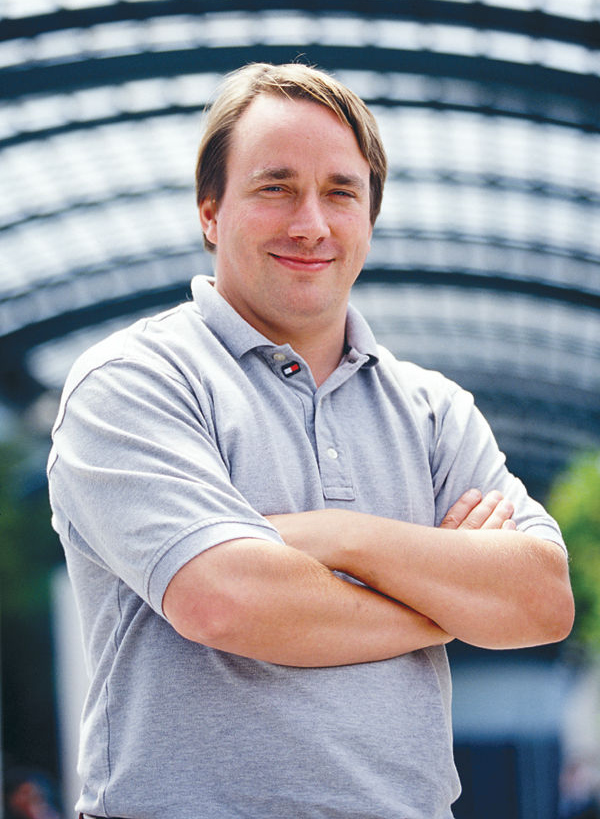
\includegraphics[width=2cm]{Figs/Linus_Torvalds}
\end{itemize}
\end{column}
\begin{column}{.2\textwidth}

\includegraphics[width=2cm]{Figs/SVN} \newline \newline

\includegraphics[width=2cm]{Figs/Git-logo}
\end{column}
\end{columns}
\end{frame}


\begin{frame}[fragile]{What is git?}
\begin{columns}[T]
\begin{column}{.8\textwidth}
\end{column}
\begin{column}{.2\textwidth}

\includegraphics[width=2cm]{Figs/Git-logo}
\end{column}
\end{columns}
\begin{itemize}
\item Git is just system of version control
\item By default it is used through a terminal
\includegraphics[width=4cm]{Figs/git/status}
\item Git has projects with multiple documents called repositories (or repos)
\item It then has a tree structure to manage the versions of the repository 
\end{itemize}
\end{frame}


\begin{frame}[fragile]{Tree structure?}
\begin{columns}[T]
\begin{column}{.8\textwidth}
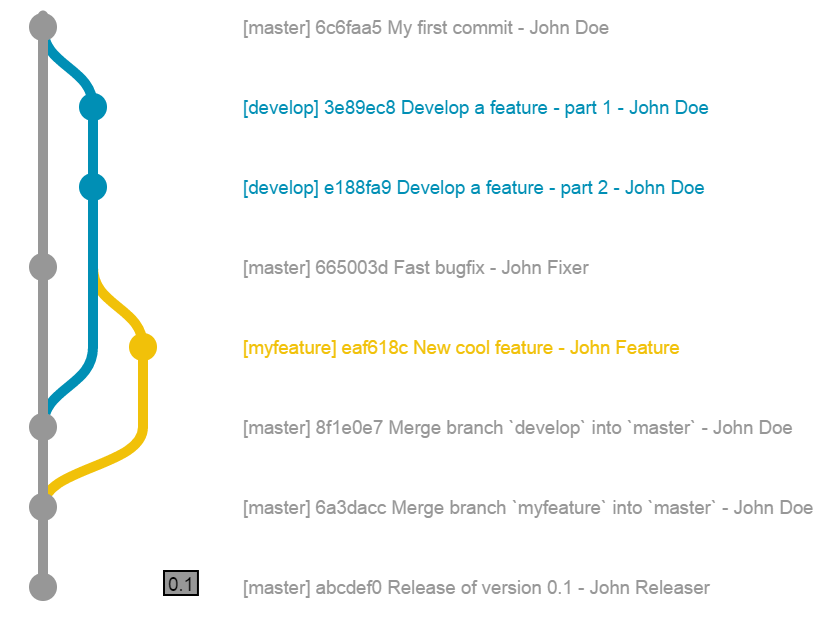
\includegraphics[width=9cm]{Figs/git/tree}
\end{column}
\begin{column}{.2\textwidth}

\includegraphics[width=2cm]{Figs/Git-logo} \newline \newline
The master branch is in grey with colour branches coming of and then being merged back
\end{column}
\end{columns}
\end{frame}


\begin{frame}[fragile]{Key commands?}
\begin{columns}[T]
\begin{column}{.8\textwidth}
In the terminal interface there are some useful commands:
\end{column}
\begin{column}{.2\textwidth}

\includegraphics[width=2cm]{Figs/Git-logo}
\end{column}
\end{columns}
\begin{itemize}
\item \textit{init} - initialise a repo
\item \textit{status} - tells you if you have flies out of sync with the current version
\item \textit{commit} - adds commits to the current version - a change with a comment and an ID
\item \textit{add} - adds new files and current commit
\item \textit{remove} - removes files and current commit
\item \textit{push} - pushes commits to an online repo (only if using a git platform)
\item \textit{pull} - pulls commits from an online platform (only if using a git platform)
\end{itemize}
\end{frame}


{%
\setbeamertemplate{frame footer}{(xkcd)}
{\setbeamercolor{palette primary}{fg=gray, bg=gray}
\begin{frame}[standout]

\includegraphics[width=6.5cm]{Figs/xkcd}
\end{frame}
}

\setbeamertemplate{frame footer}{ }
\section{Platform}


\begin{frame}[fragile]{Which platform?}
You can just use git with the terminal on your PC or you can store work on an online repository managing platform, the most popular of these are GitHub and Bitbucket\\
\begin{columns}[T]
\begin{column}{.8\textwidth}
\smartdiagram[bubble diagram]{Effective\\ version\\ control,
System, Storage/\\platform, UI/\\interface}
\end{column}
\begin{column}{.2\textwidth}

\includegraphics[width=2cm]{Figs/git/Octocat} \newline \newline \newline 

\includegraphics[width=2cm]{Figs/git/Bitbucket}
\end{column}
\end{columns}
\end{frame}


\begin{frame}[fragile]{Why not just store the repository on Dropbox?}
You can and it would be baked up and sharable, but there are problems:\\
\begin{columns}[T]
\begin{column}{.8\textwidth}
\begin{itemize}
\item You can run into Dropbox syncing and git version control clashes
\item If you share the files with a collaborator they aren’t identified separately to you
\item You or a collaborator can completely mess up the git system (mostly by deleting the records in the `.git' folder)
\item If you do you can't just re download
\end{itemize}
\end{column}
\begin{column}{.2\textwidth}

\includegraphics[width=2cm]{Figs/git/Dropbox}
\end{column}
\end{columns}
\end{frame}


\begin{frame}[fragile]{Which platform?}
\begin{columns}[T]
\begin{column}{.8\textwidth}
\textbf{Bitbucket}
\begin{itemize}
\item Allows unlimited public or private repositories
\item Charges per collaborators over 5 on those repositories 
\item 1GB storage for \textbf{large} flies all repositories, 5GB if using a .ac email
\end{itemize}
\textbf{GitHub}
\begin{itemize}
\item Has unlimited public repositories 
\item With unlimited collaborators
\item Pay for private repositories
\item However as a student or academic you can sign up for free private repositories
\item GitHub is about $\times$4 more popular than Bitbucket
\end{itemize}
\end{column}
\begin{column}{.2\textwidth}

\includegraphics[width=2cm]{Figs/git/Bitbucket} \newline \newline \newline \newline 

\includegraphics[width=2cm]{Figs/git/Octocat}
\end{column}
\end{columns}
\end{frame}



\section{UI}


\begin{frame}[fragile]{Which UI?}
You can just use git with the terminal but there is a friendlier interface\\
\begin{columns}[T]
\begin{column}{.8\textwidth}
\smartdiagram[bubble diagram]{Effective\\ version\\ control,
System, Storage/\\platform, UI/\\interface}
\end{column}
\begin{column}{.2\textwidth}

\includegraphics[width=2cm]{Figs/git/terminal} \newline \newline

\includegraphics[width=2cm]{Figs/git/gitdesktop} \newline \newline

\includegraphics[width=2cm]{Figs/git/Sourcetree}
\end{column}
\end{columns}
\end{frame}


\begin{frame}[fragile]{Which UI?}
\begin{columns}[T]
\begin{column}{.8\textwidth}
\textbf{The Terminal\\}
You can just use the terminal with the raw git commands as seen before... but:
\begin{itemize}
\item If you are not using it anyway or are happy using it a graphical UI is nice 
\item You don't need to remember commands or repo names 
\item You need to install git for widows \url{https://git-scm.com/download/win}
\end{itemize}
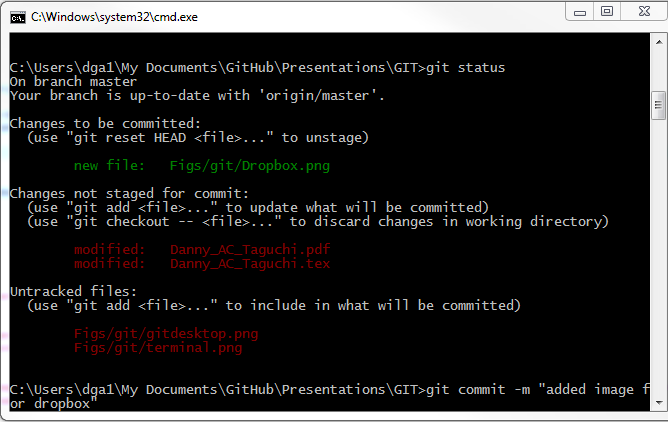
\includegraphics[width=6cm]{Figs/git/terminaluse}
\end{column}
\begin{column}{.2\textwidth}

\includegraphics[width=2cm]{Figs/git/terminal} \newline \newline \newline 
\end{column}
\end{columns}
\end{frame}



\begin{frame}[fragile]{Which UI?}
\begin{columns}[T]
\begin{column}{.8\textwidth}
\textbf{Git Desktop\\}
The essayist to use and most popular UI is git desktop:
\begin{itemize}
\item This is made by GitHub and integrates very well with GitHub or local (on pc) repositories
\item It will work with other hosting platforms but less easily
\item Is the essayist to use!
\item Will install git for widows \url{https://git-scm.com/download/win}
\end{itemize}
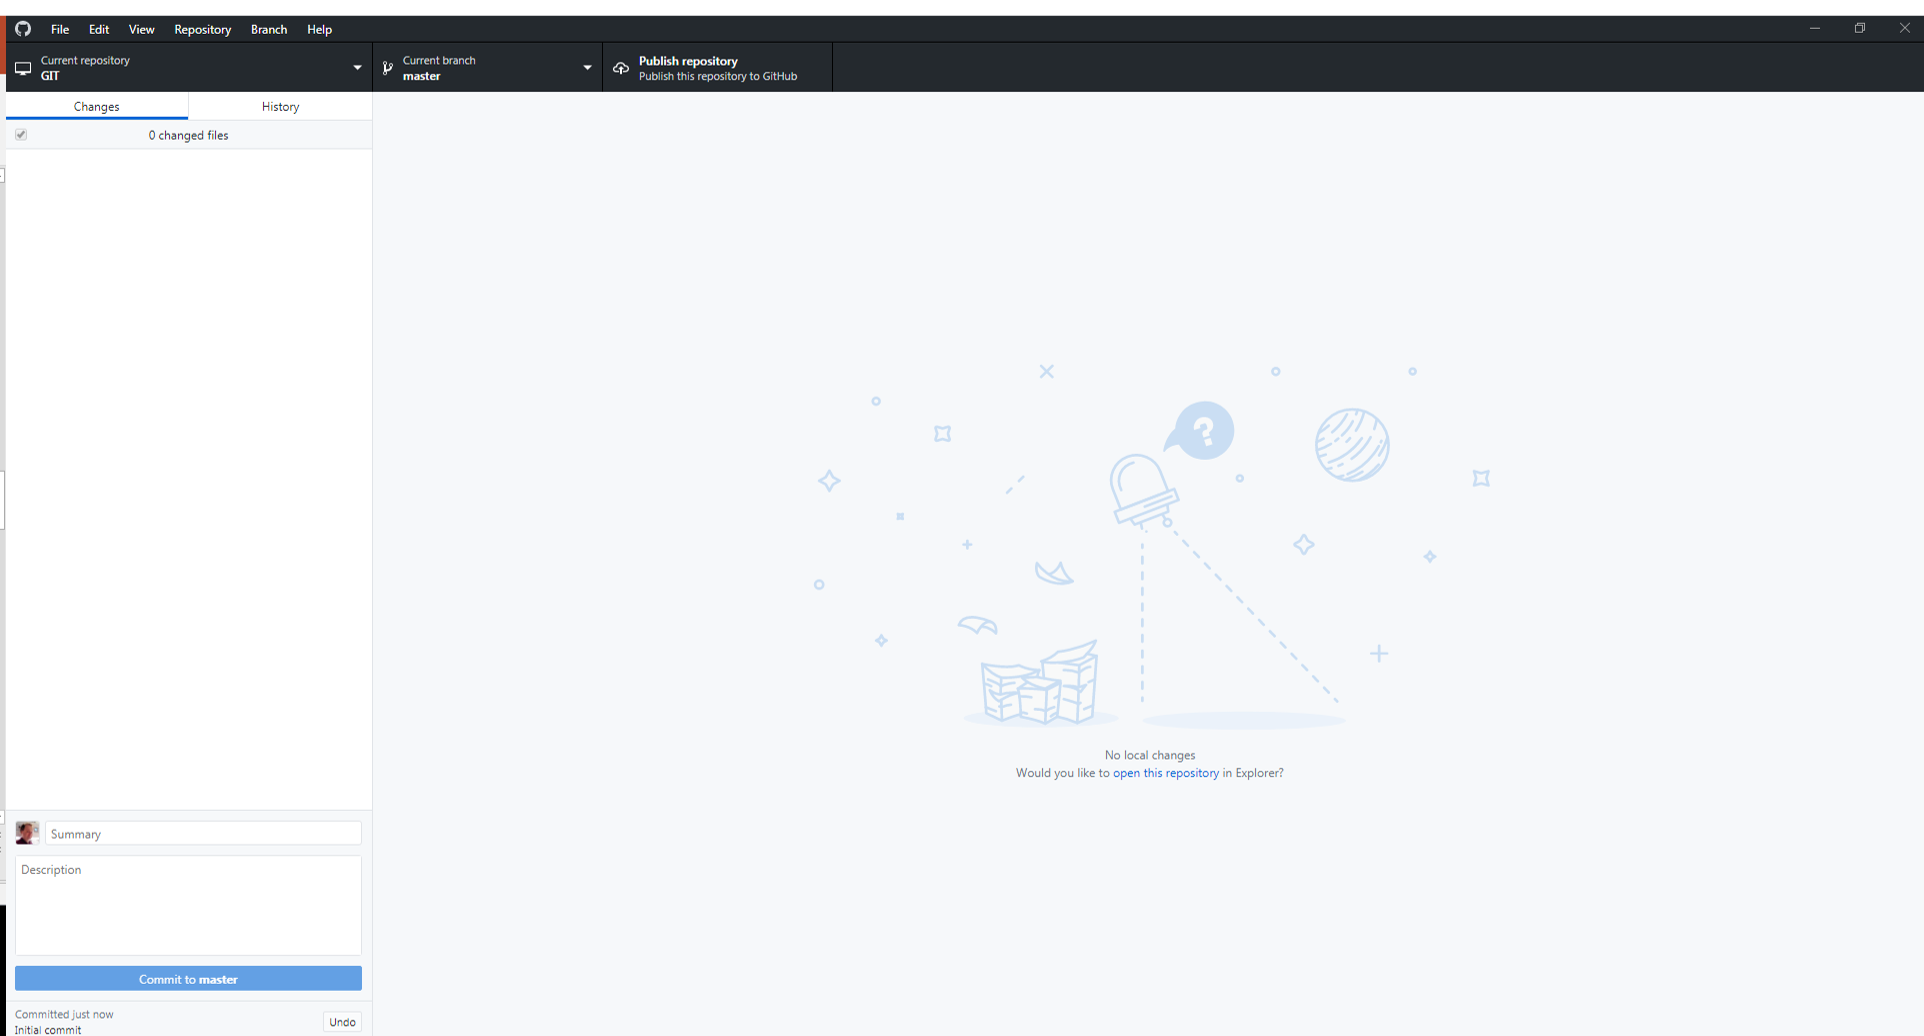
\includegraphics[width=8cm]{Figs/GHD/outline_02}
\end{column}
\begin{column}{.2\textwidth}

\includegraphics[width=2cm]{Figs/git/gitdesktop} \newline \newline \newline 
\end{column}
\end{columns}
\end{frame}


\begin{frame}[fragile]{Which UI?}
\begin{columns}[T]
\begin{column}{.8\textwidth}
\textbf{Sourcetree\\}
\begin{itemize}
\item Sourcetree is owned by atlassian who ouns Bitbucket
\item It will work with other hosting platforms easily
\item It has more complex controls
\item Will install git for widows \url{https://git-scm.com/download/win}
\end{itemize}
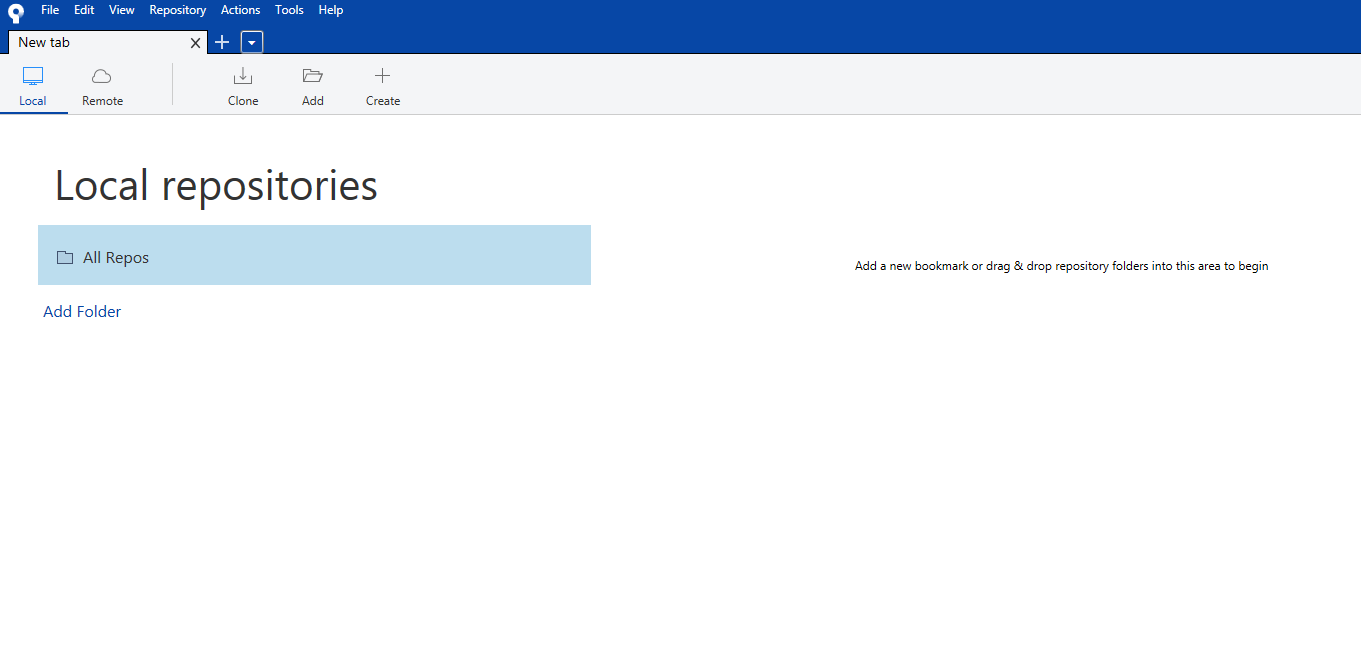
\includegraphics[width=8cm]{Figs/ST/ST_00} 
\end{column}
\begin{column}{.2\textwidth}

\includegraphics[width=2cm]{Figs/git/Sourcetree} \newline \newline \newline 
\end{column}
\end{columns}
\end{frame}


\section{Using git}


\begin{frame}[fragile]{How to use git}
\begin{columns}[T]
\begin{column}{.8\textwidth}
\textbf{This will assume use of GitHub and GitDesktop\\}
\url{https://desktop.github.com} \newline \newline 
Following is a brief demonstration of the interface
\end{column}
\begin{column}{.2\textwidth}

\includegraphics[width=2cm]{Figs/git/Octocat} \newline \newline \newline 

\includegraphics[width=2cm]{Figs/git/gitdesktop}
\end{column}
\end{columns}
\end{frame}


\begin{frame}[fragile]{Adding a new repository}
\begin{columns}[T]
\begin{column}{.12\textwidth}
\end{column}
\begin{column}{.88\textwidth}
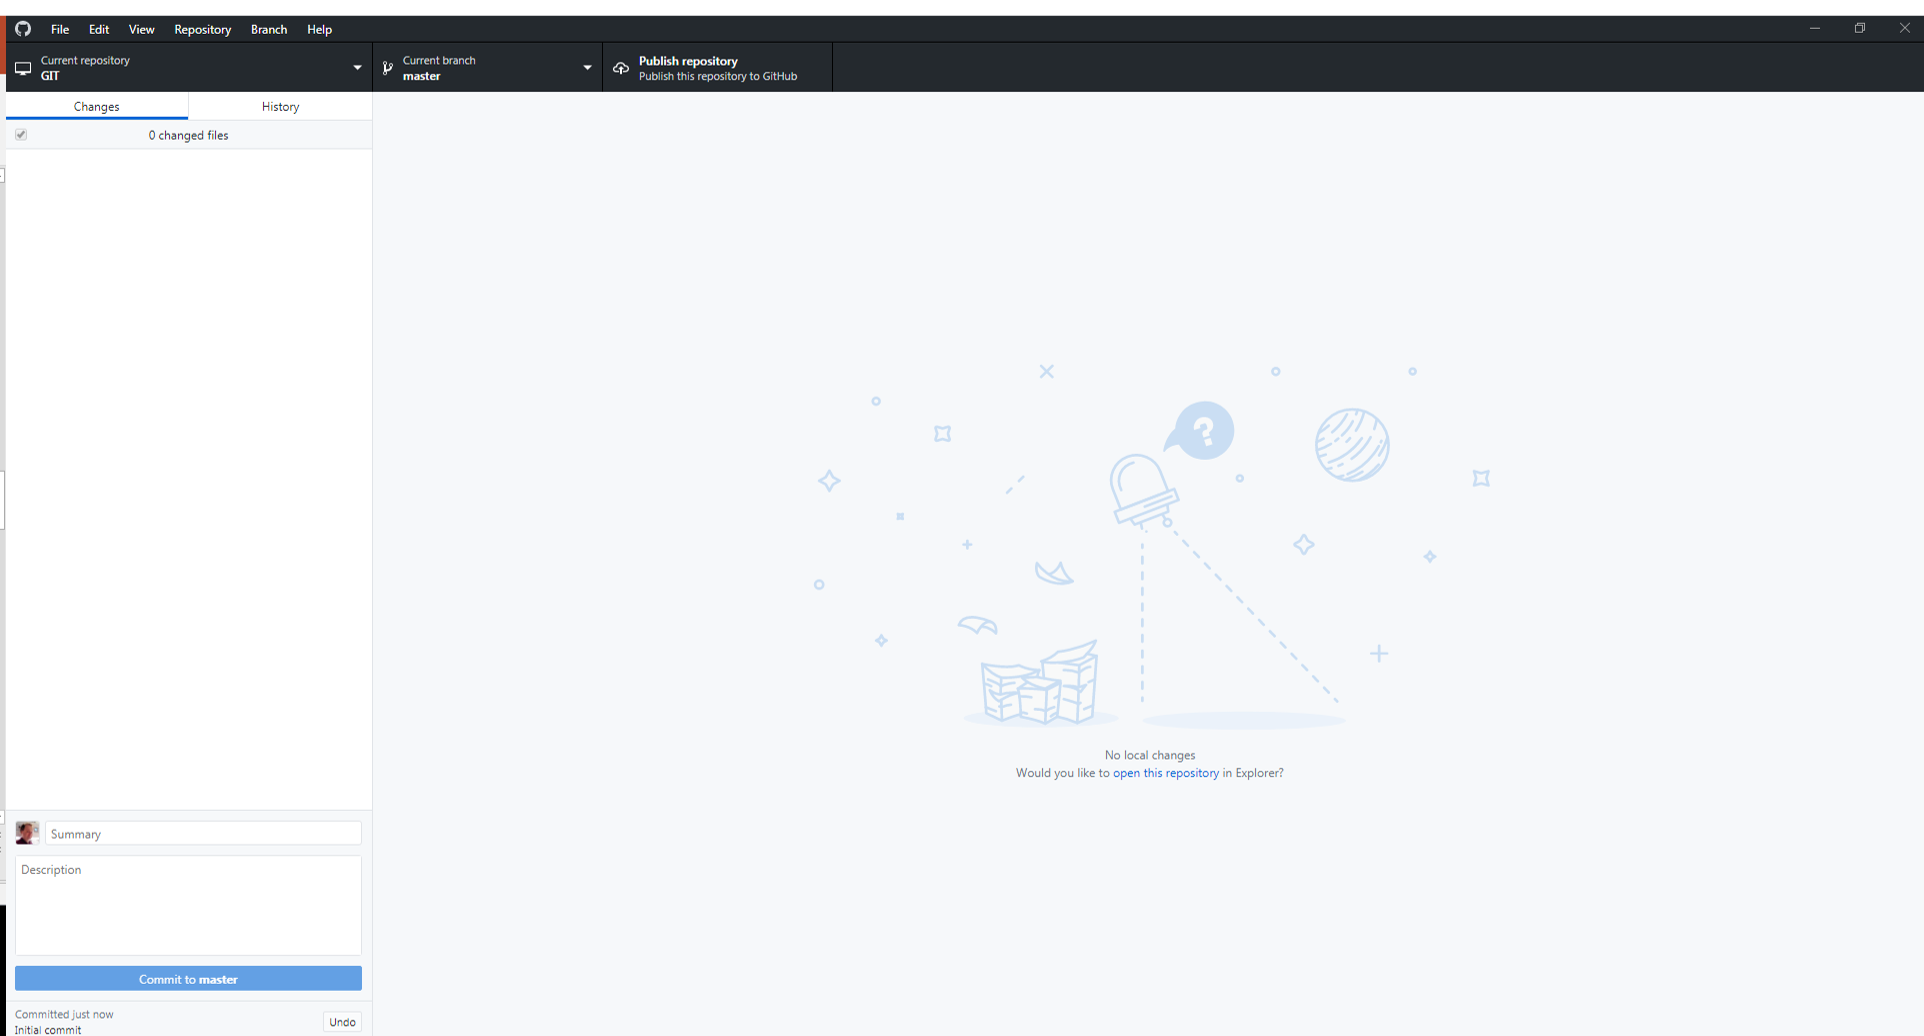
\includegraphics[width=10cm]{Figs/GHD/outline_02}
\end{column}
\end{columns}
\end{frame}



\begin{frame}[fragile]{Adding a new repository}
\begin{columns}[T]
\begin{column}{.12\textwidth}
\end{column}
\begin{column}{.88\textwidth}
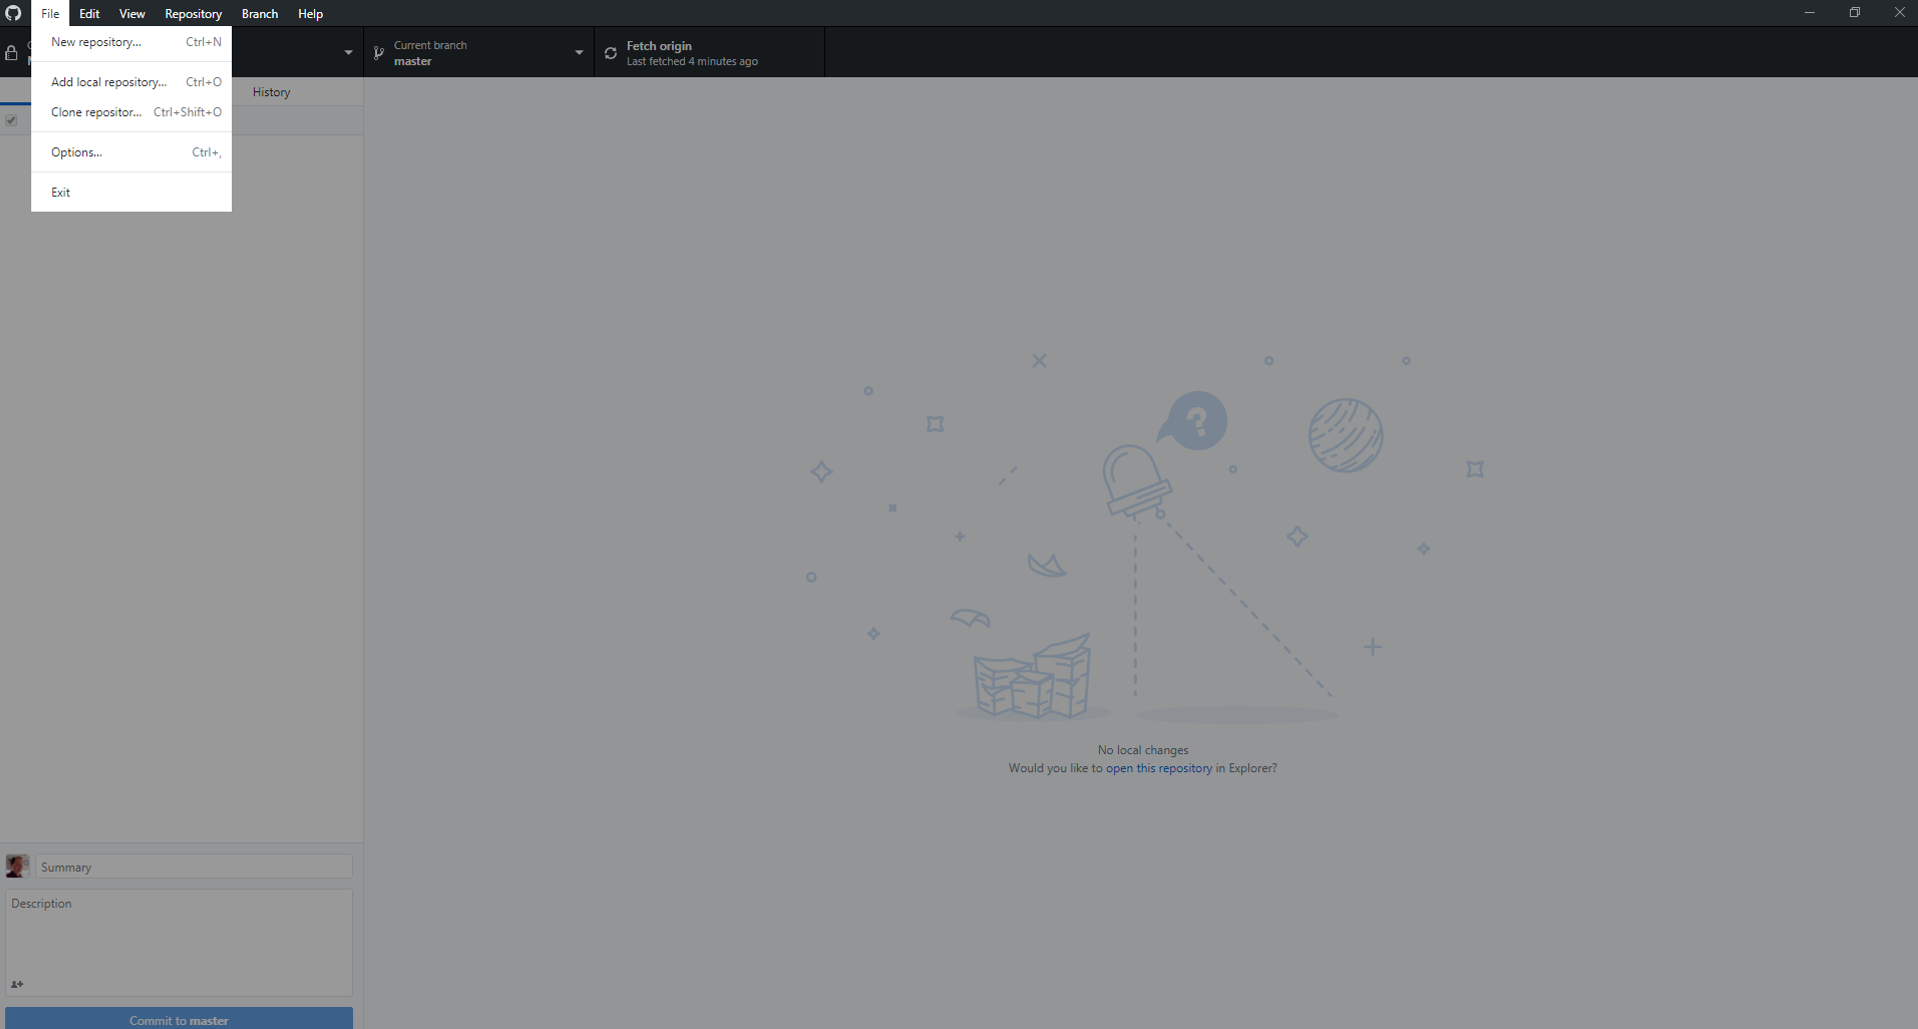
\includegraphics[width=10cm]{Figs/GHD/outline_01}
\end{column}
\end{columns}
\end{frame}


\begin{frame}[fragile]{Adding a new repository}
\begin{columns}[T]
\begin{column}{.12\textwidth}
\small This makes a totally new repository (with no `.git' folder)
\end{column}
\begin{column}{.88\textwidth}
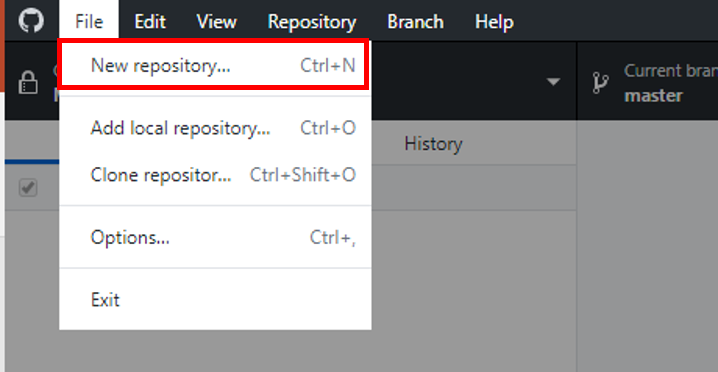
\includegraphics[width=10cm]{Figs/GHD/menu_02}
\end{column}
\end{columns}
\end{frame}

\begin{frame}[fragile]{Adding a new repository}
\begin{columns}[T]
\begin{column}{.12\textwidth}
\small adds an existing repository (with a `.git' folder)
\end{column}
\begin{column}{.88\textwidth}
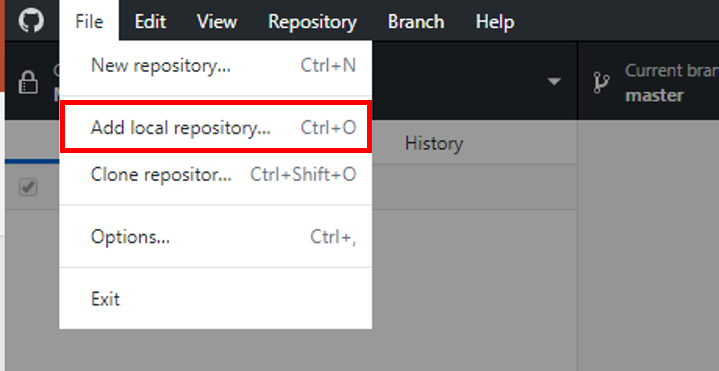
\includegraphics[width=10cm]{Figs/GHD/menu_03}
\end{column}
\end{columns}
\end{frame}

\begin{frame}[fragile]{Adding a new repository}
\begin{columns}[T]
\begin{column}{.12\textwidth}
\small Copies an online repository to the PC
\end{column}
\begin{column}{.88\textwidth}
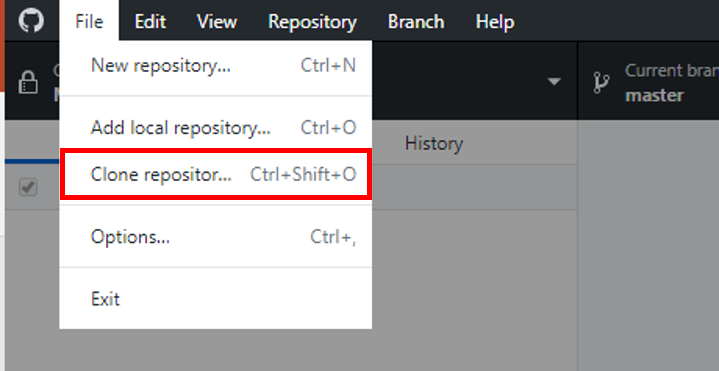
\includegraphics[width=10cm]{Figs/GHD/menu_04}
\end{column}
\end{columns}
\end{frame}

\begin{frame}[fragile]{Adding a new repository}
\begin{columns}[T]
\begin{column}{.2\textwidth}
\small new repository menu
\end{column}
\begin{column}{.8\textwidth}
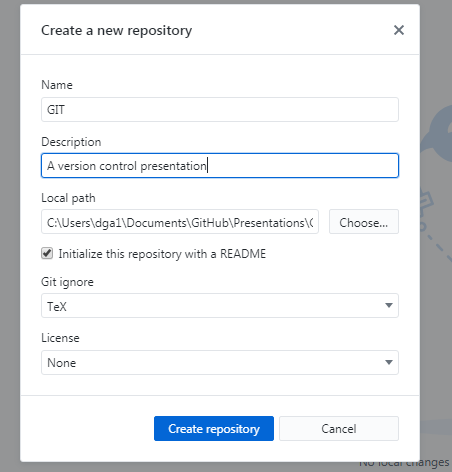
\includegraphics[width=8cm]{Figs/GHD/new_repo_00}
\end{column}
\end{columns}
\end{frame}


\begin{frame}[fragile]{Adding a new repository}
\begin{columns}[T]
\begin{column}{.2\textwidth}
\end{column}
\begin{column}{.8\textwidth}
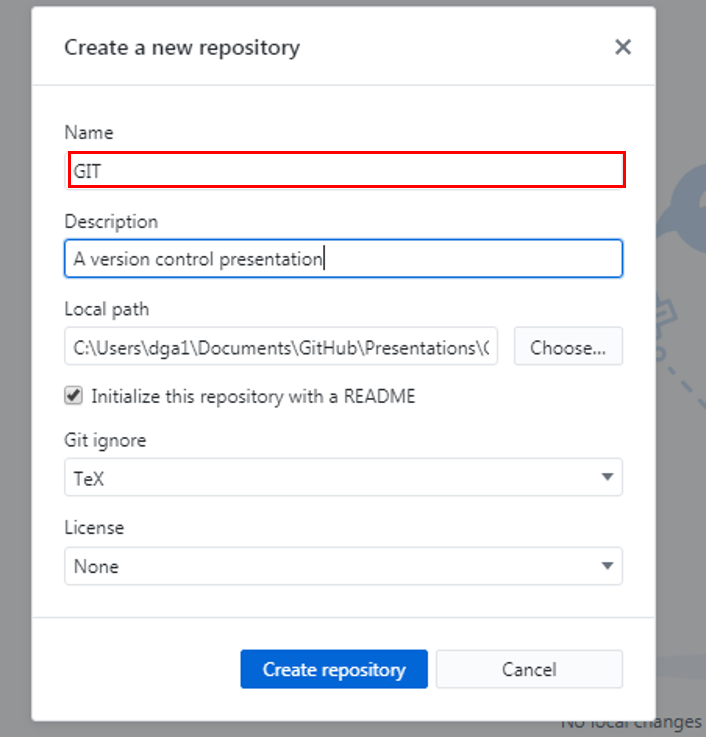
\includegraphics[width=8cm]{Figs/GHD/new_repo_01}
\end{column}
\end{columns}
\end{frame}

\begin{frame}[fragile]{Adding a new repository}
\begin{columns}[T]
\begin{column}{.2\textwidth}
\end{column}
\begin{column}{.8\textwidth}
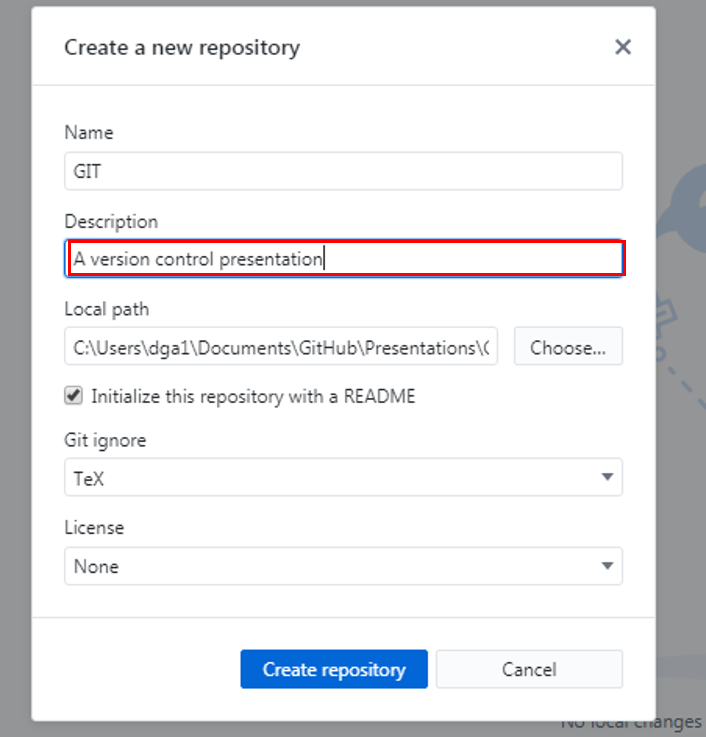
\includegraphics[width=8cm]{Figs/GHD/new_repo_02}
\end{column}
\end{columns}
\end{frame}

\begin{frame}[fragile]{Adding a new repository}
\begin{columns}[T]
\begin{column}{.2\textwidth}
\small The folder \textbf{in which} to store the git repository folder.
\end{column}
\begin{column}{.8\textwidth}
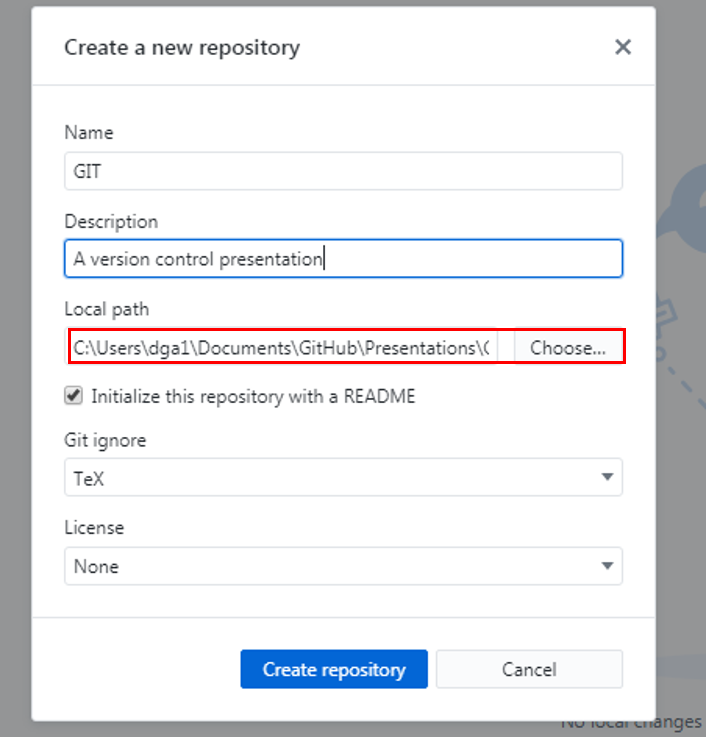
\includegraphics[width=8cm]{Figs/GHD/new_repo_03}
\end{column}
\end{columns}
\end{frame}

\begin{frame}[fragile]{Adding a new repository}
\begin{columns}[T]
\begin{column}{.2\textwidth}
\small This will initialise the repository with a readme containing the description.
\end{column}
\begin{column}{.8\textwidth}
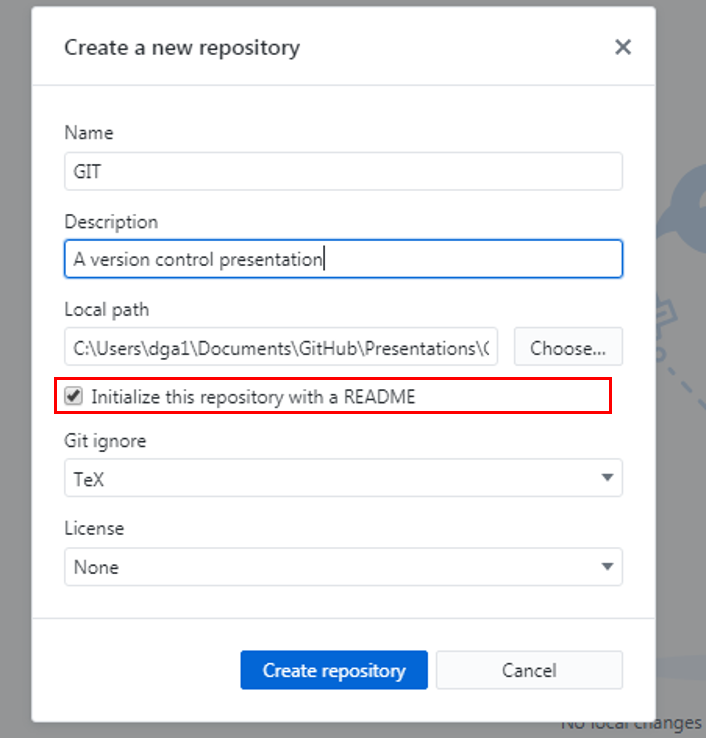
\includegraphics[width=8cm]{Figs/GHD/new_repo_04}
\end{column}
\end{columns}
\end{frame}

\begin{frame}[fragile]{Adding a new repository}
\begin{columns}[T]
\begin{column}{.2\textwidth}
\small This is a file called `.gitignore' which lists files \& folders to not version control
\end{column}
\begin{column}{.8\textwidth}
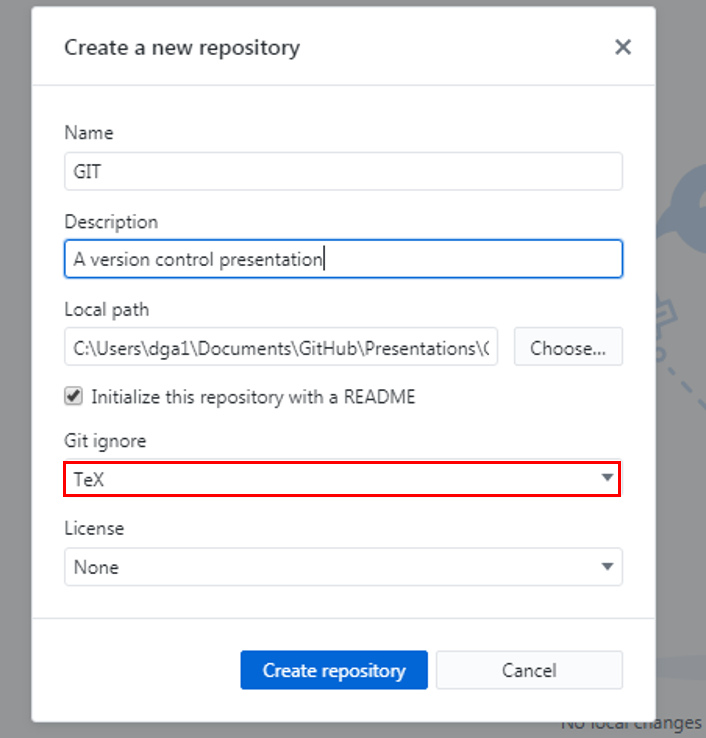
\includegraphics[width=8cm]{Figs/GHD/new_repo_05}
\end{column}
\end{columns}
\end{frame}


\begin{frame}[fragile]{Using the repository}
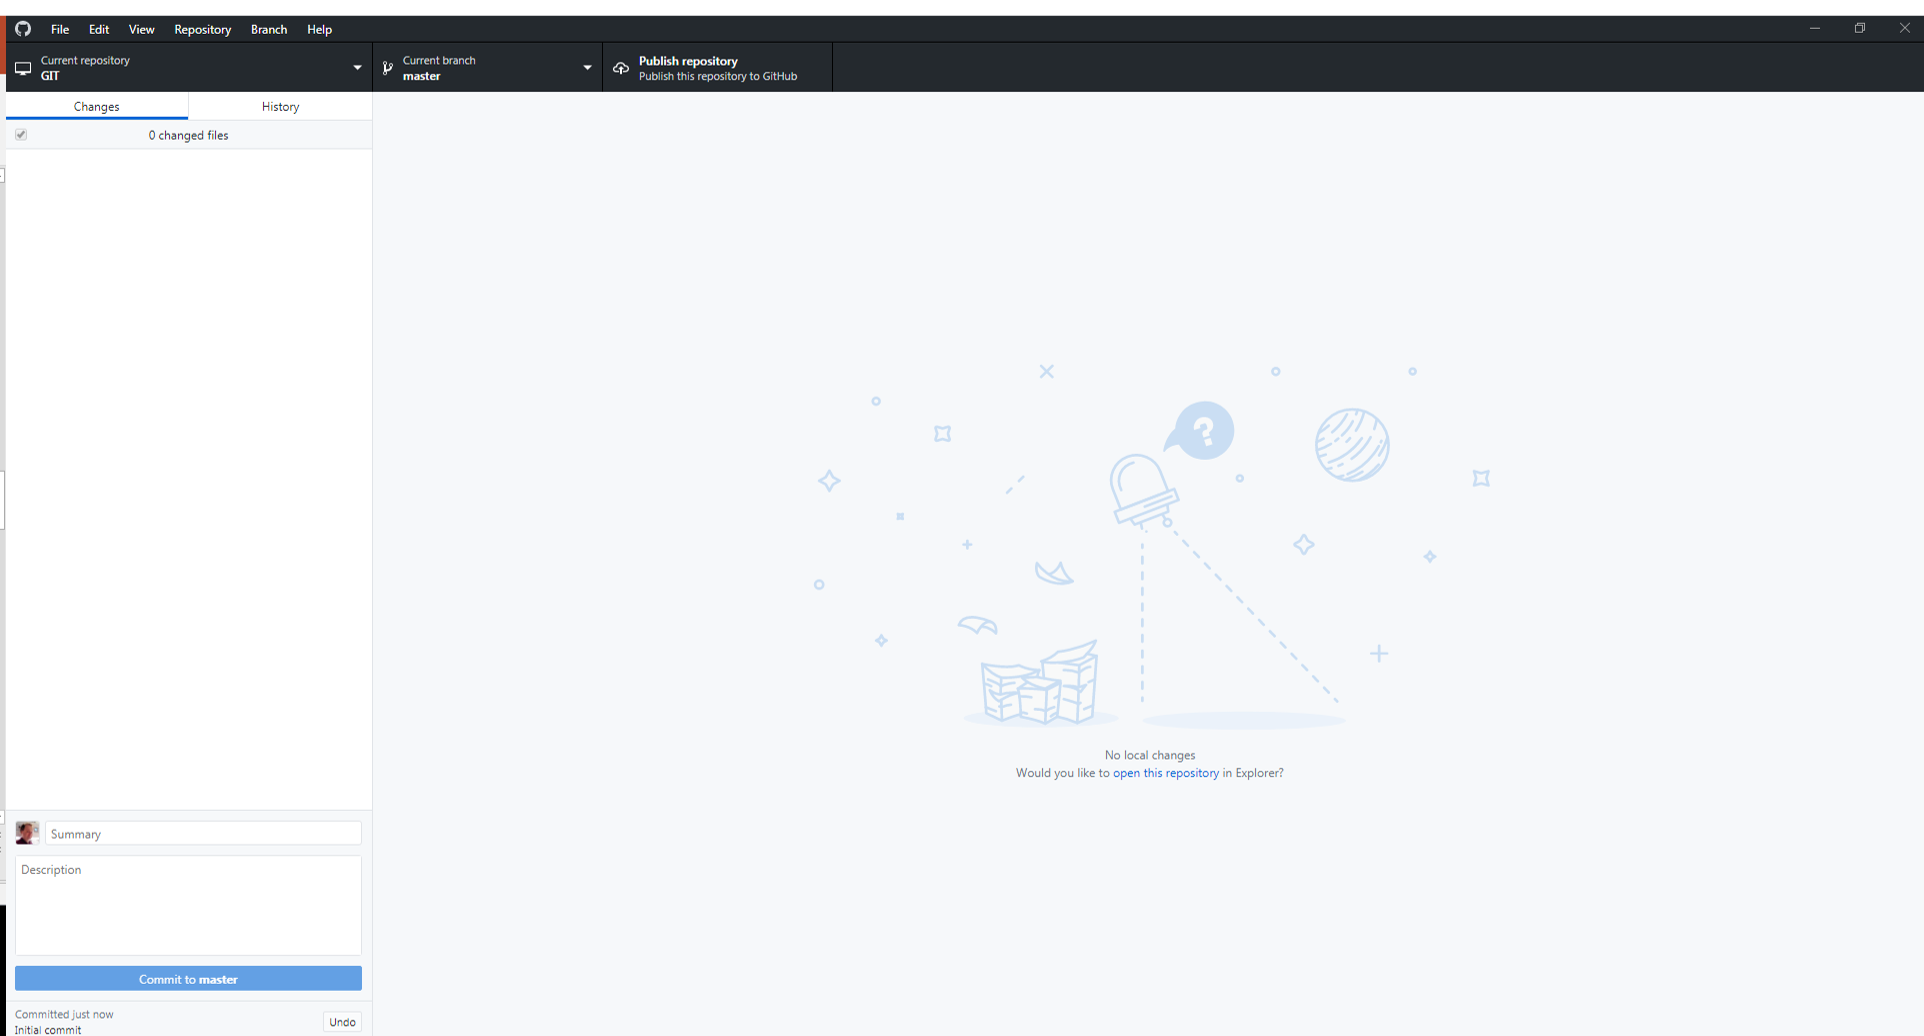
\includegraphics[width=12cm]{Figs/GHD/outline_02}
\end{frame}


\begin{frame}[fragile]{Using the repository}
\small Now we have a initial commit of the readme done
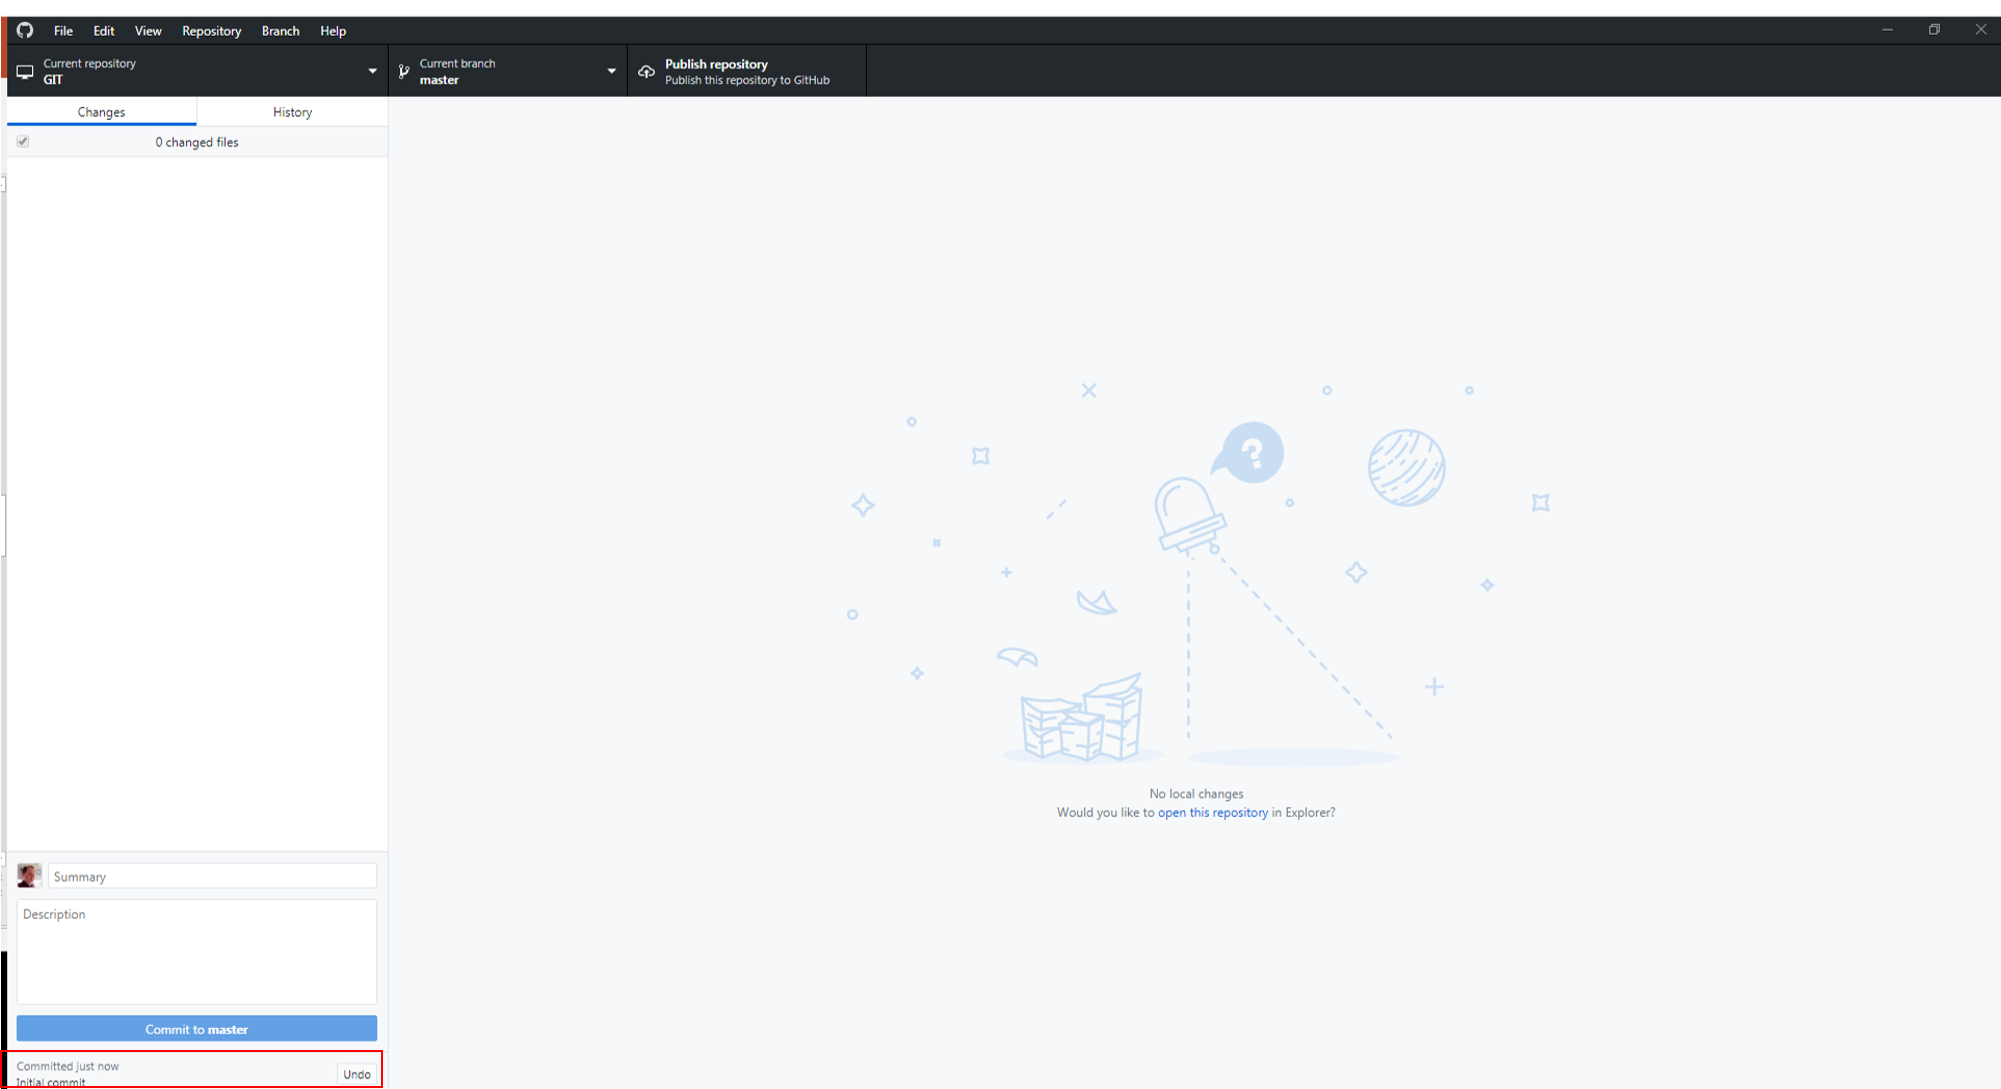
\includegraphics[width=12cm]{Figs/GHD/outline_09}
\end{frame}


\begin{frame}[fragile]{Using the repository}
\small We can carry on making local commits or publish the repository to GitHub
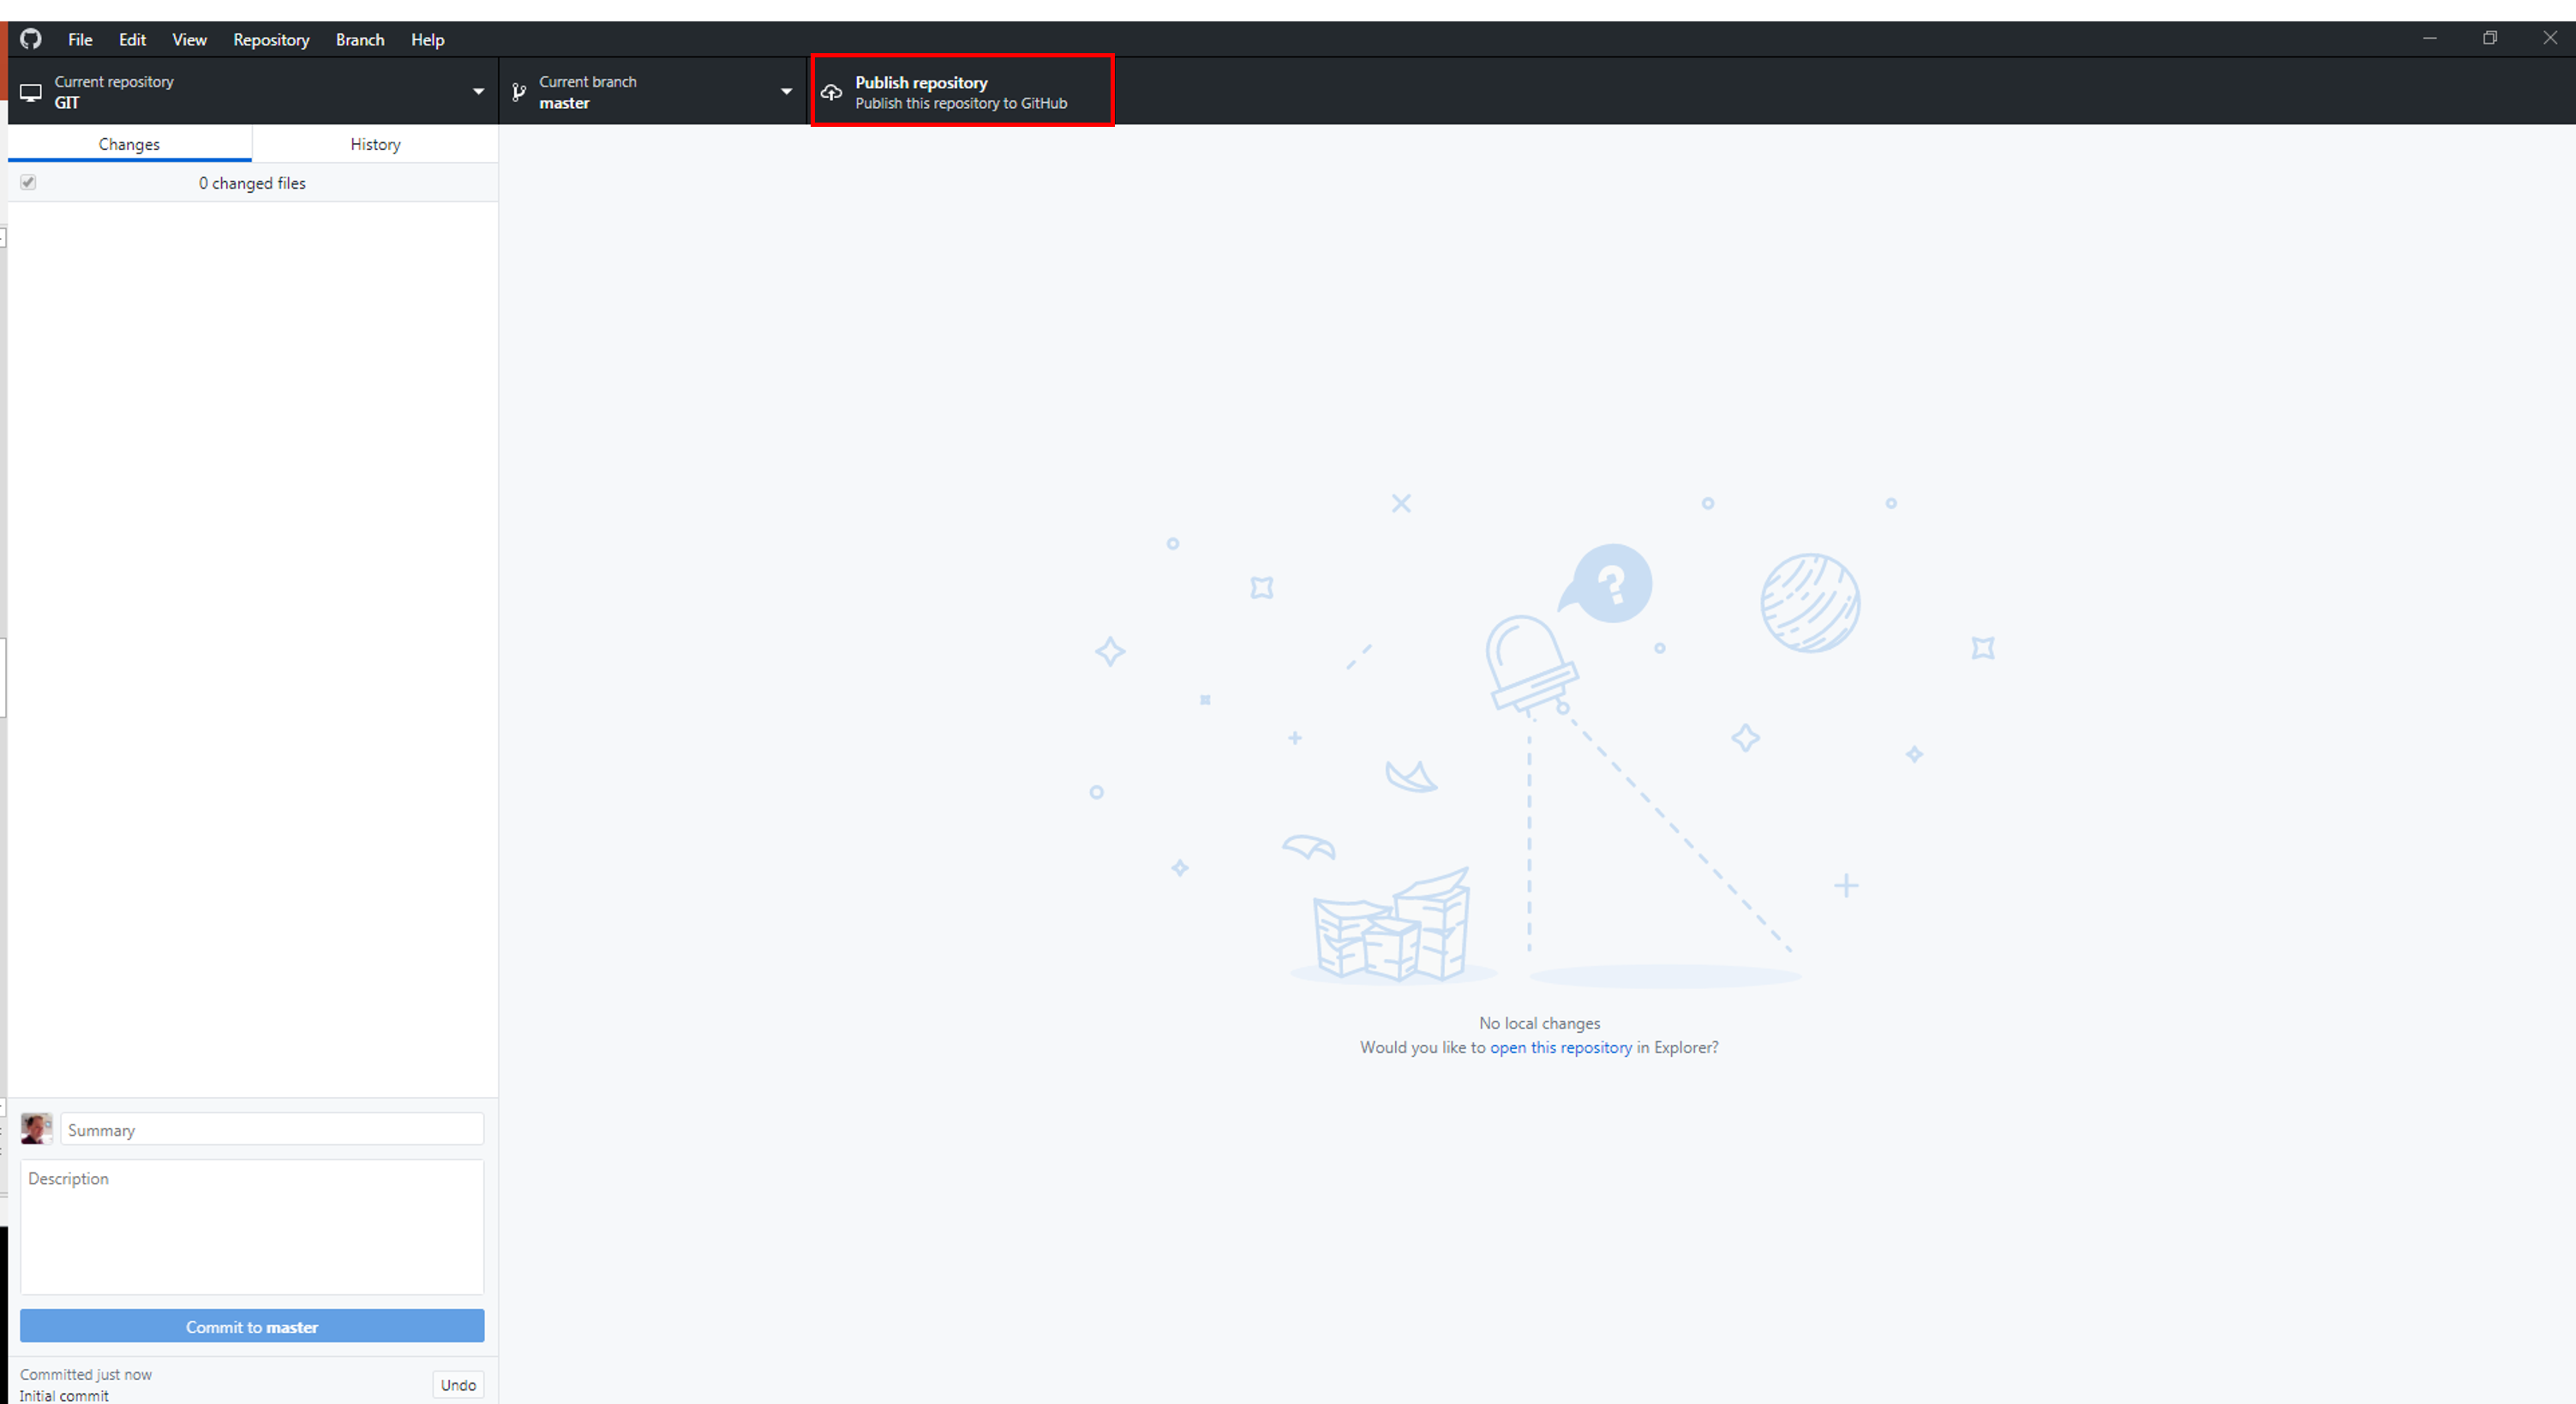
\includegraphics[width=12cm]{Figs/GHD/outline_03}
\end{frame}

\begin{frame}[fragile]{Using the repository}
\small We can publish to GitHub
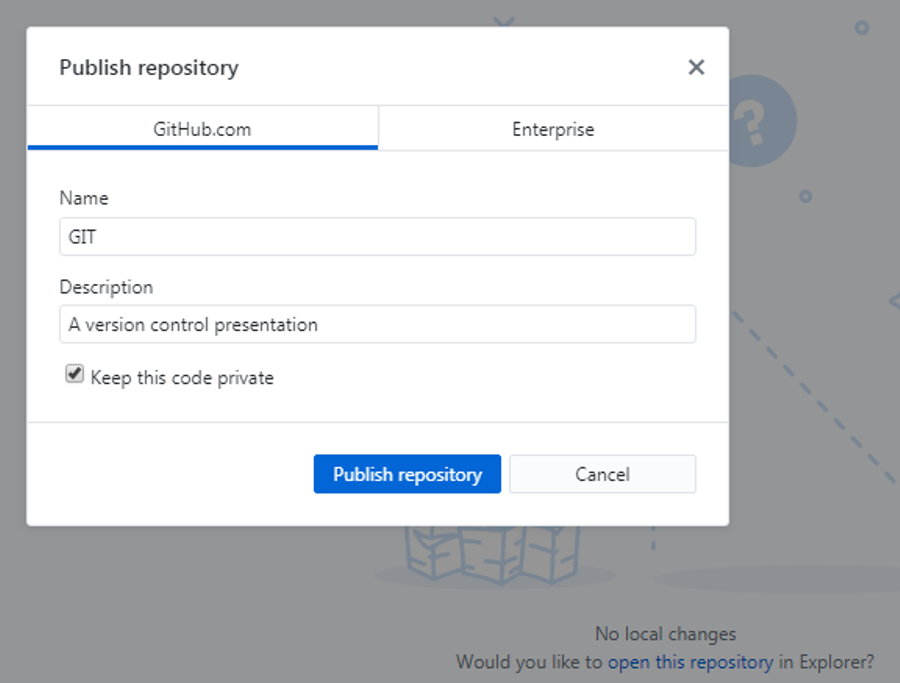
\includegraphics[width=12cm]{Figs/GHD/init_00}
\end{frame}

\begin{frame}[fragile]{Using the repository}
\small Make branches
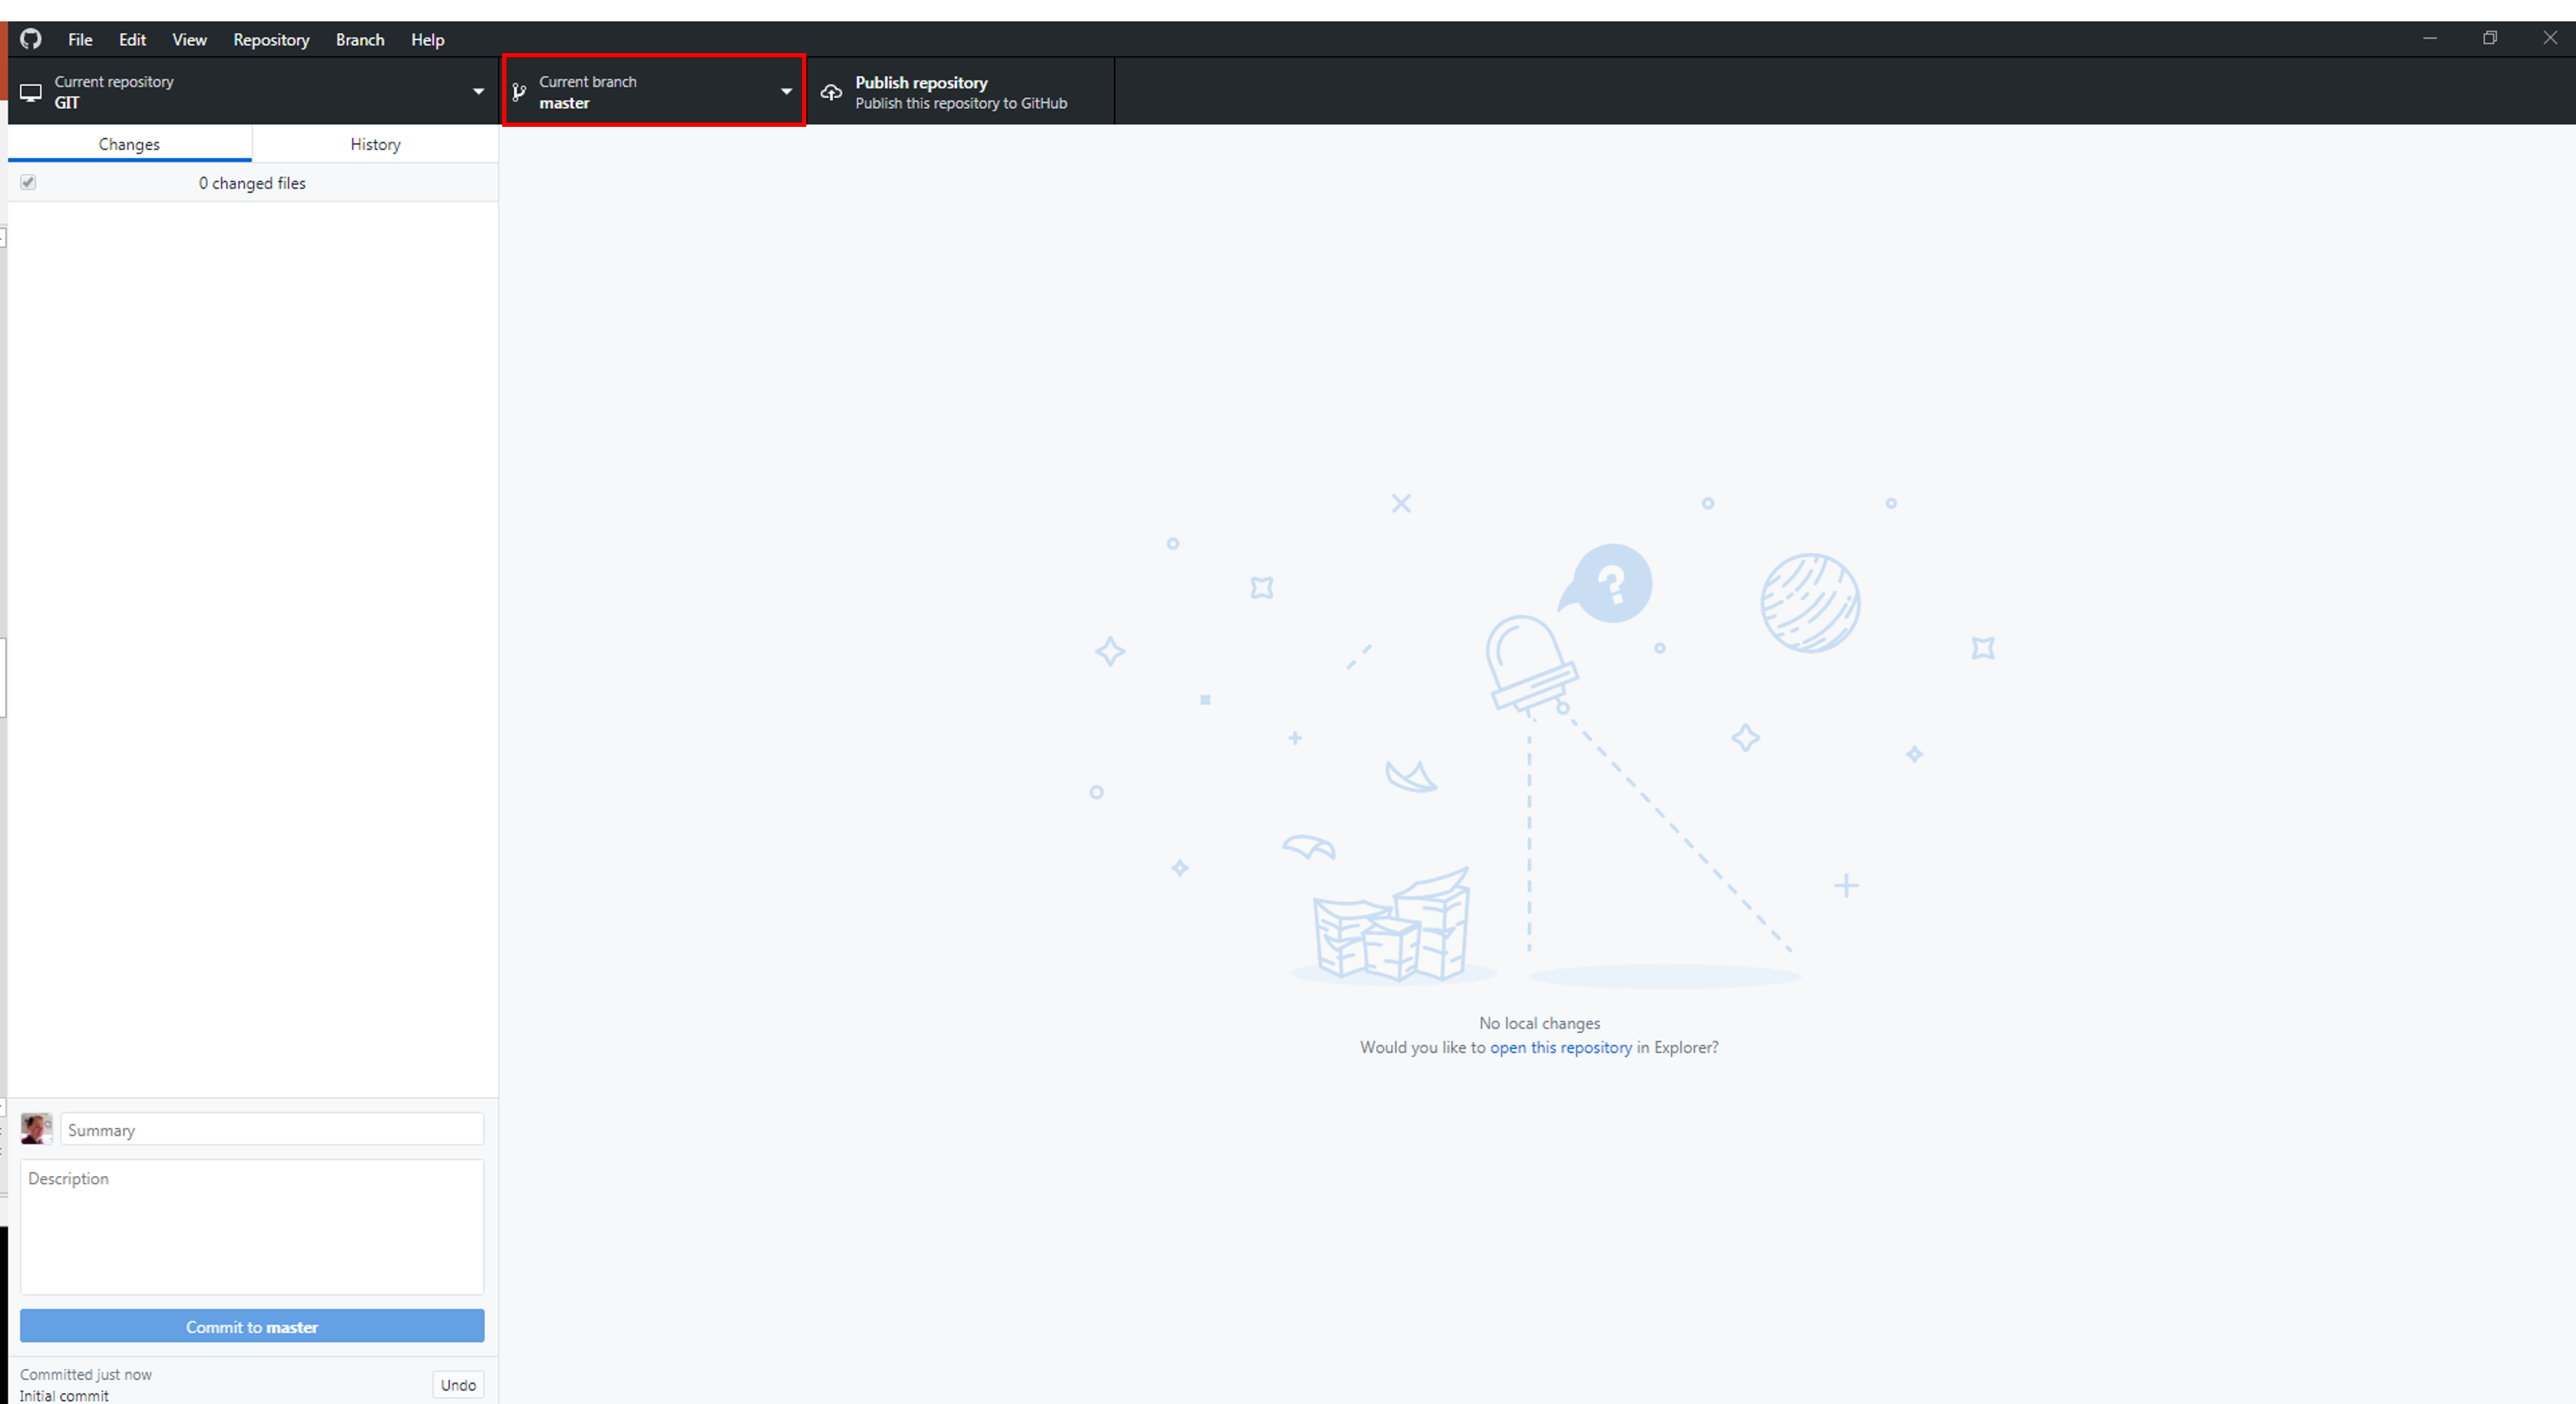
\includegraphics[width=12cm]{Figs/GHD/outline_04}
\end{frame}

\begin{frame}[fragile]{Using the repository}
\small Switch to another repository
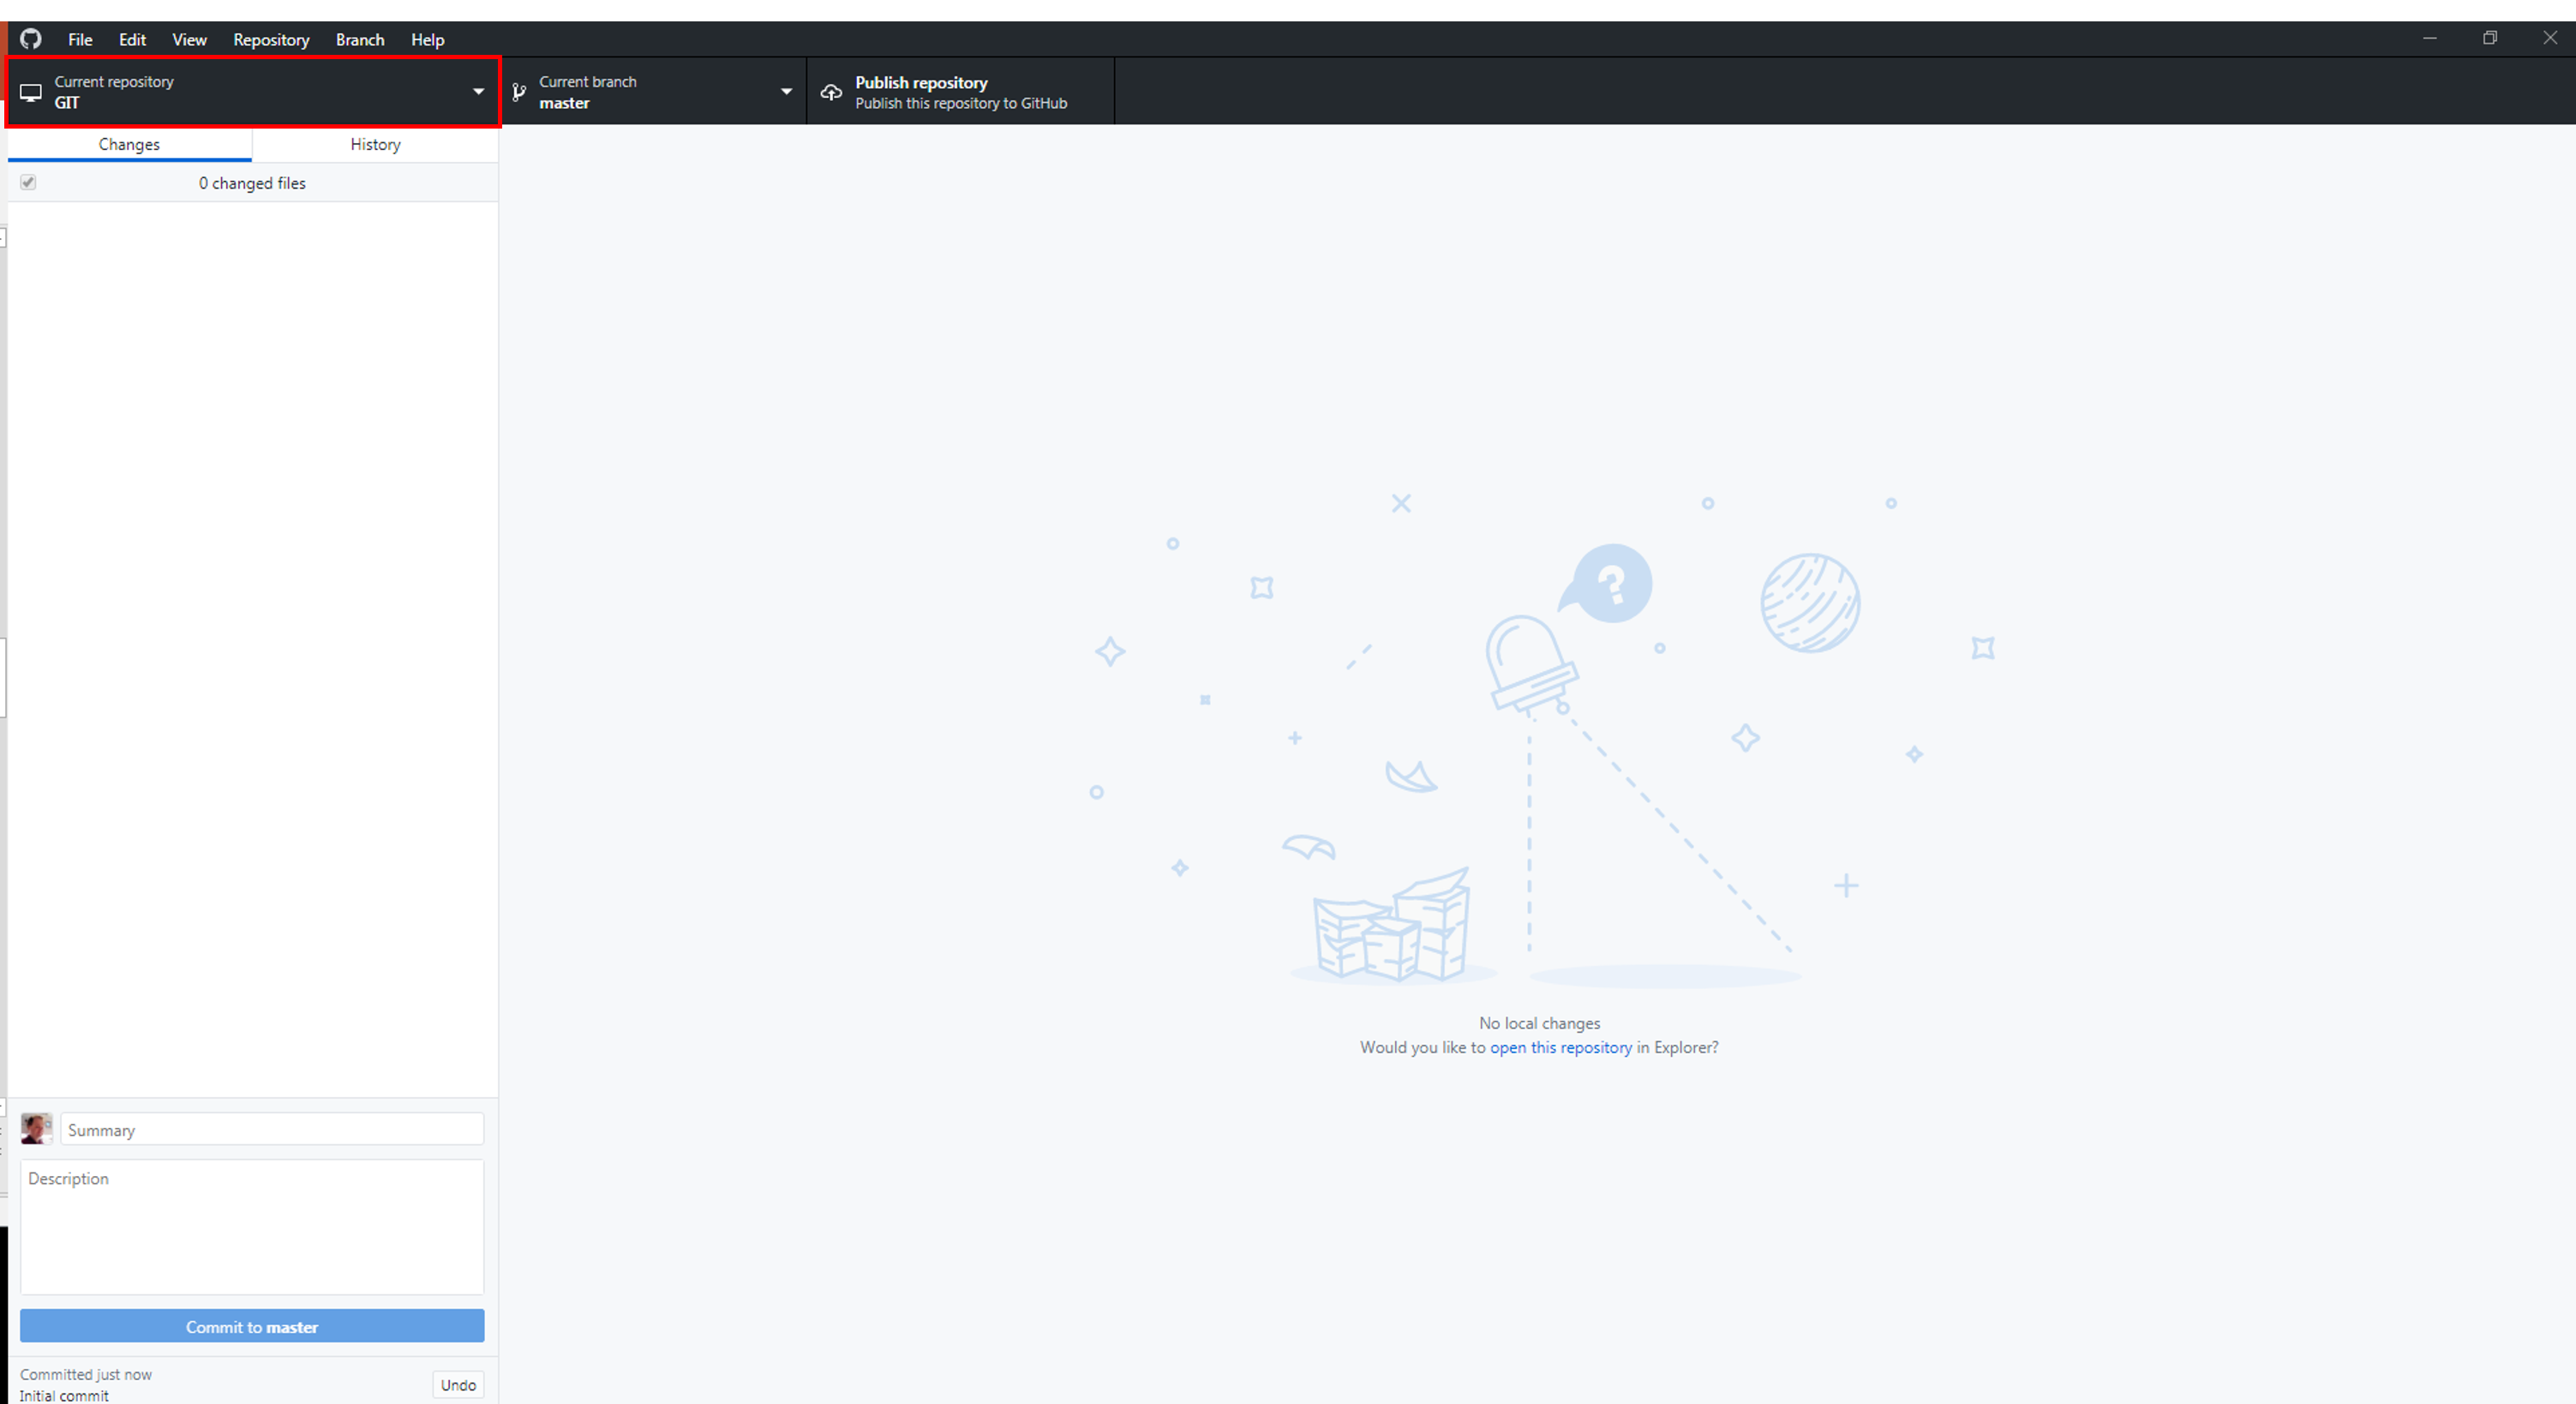
\includegraphics[width=12cm]{Figs/GHD/outline_05}
\end{frame}

\begin{frame}[fragile]{Using the repository}
\small Look at the history of this repository
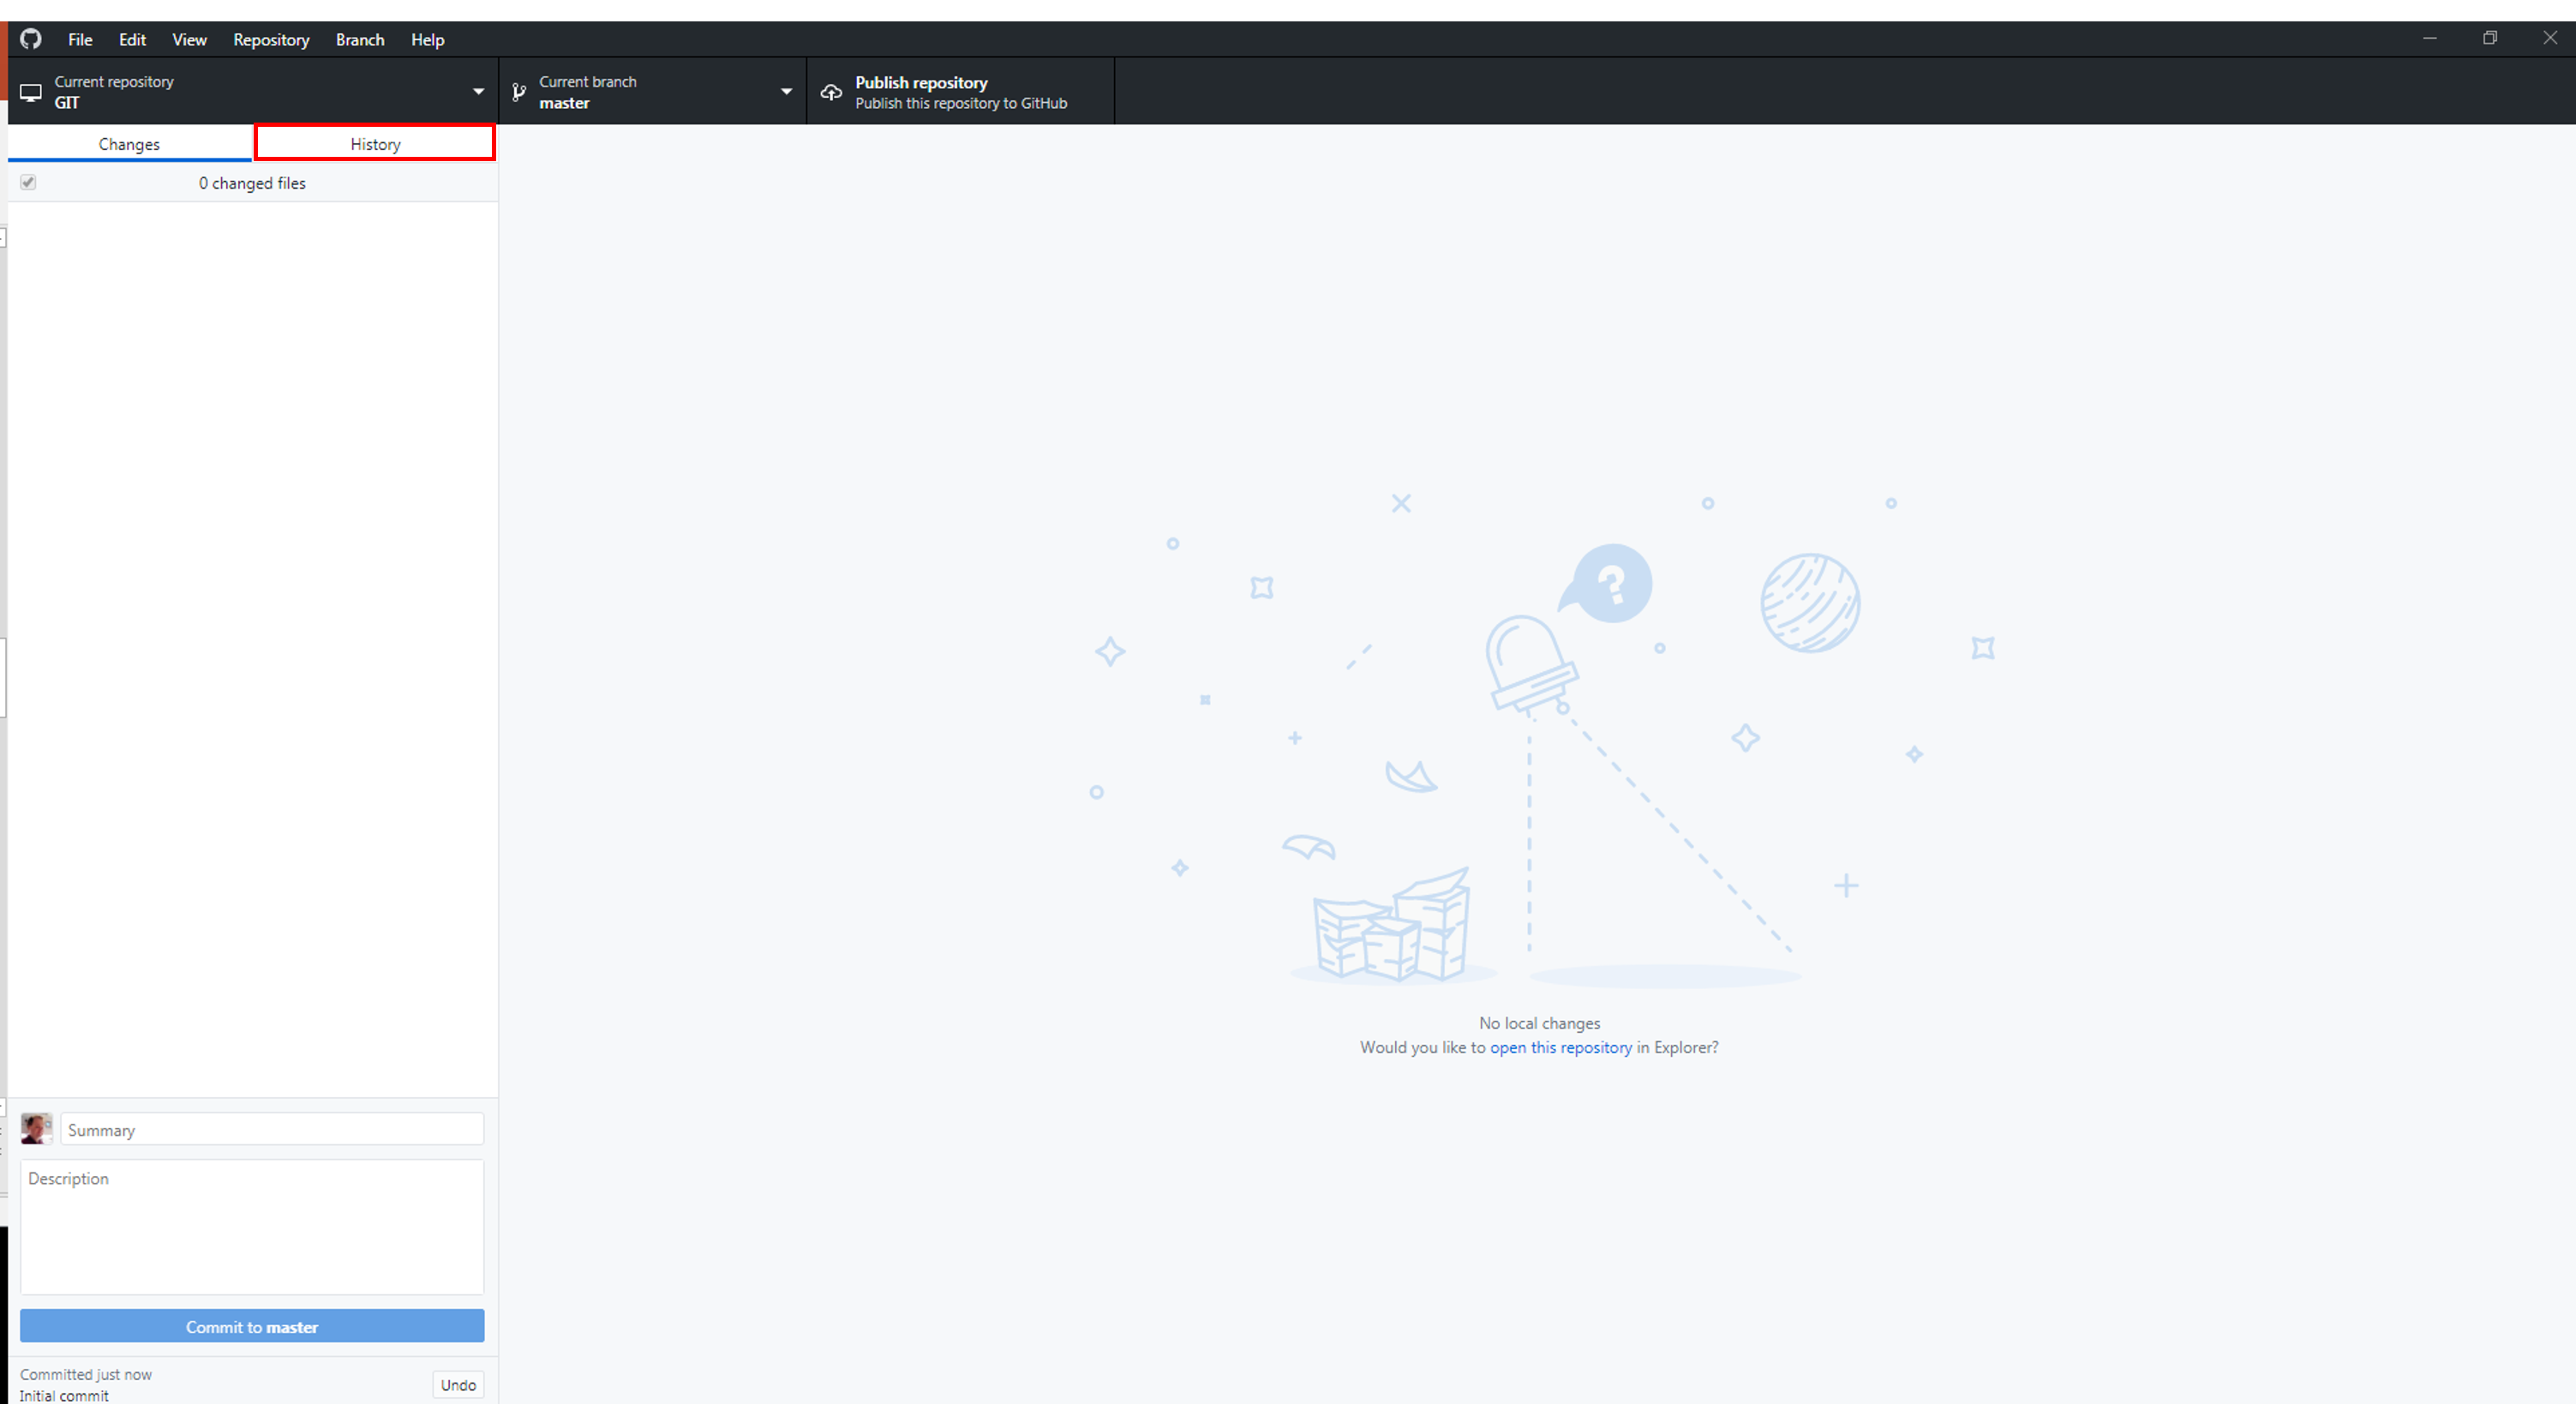
\includegraphics[width=12cm]{Figs/GHD/outline_06}
\end{frame}

\begin{frame}[fragile]{Using the repository}
\small Look at the history of this repository
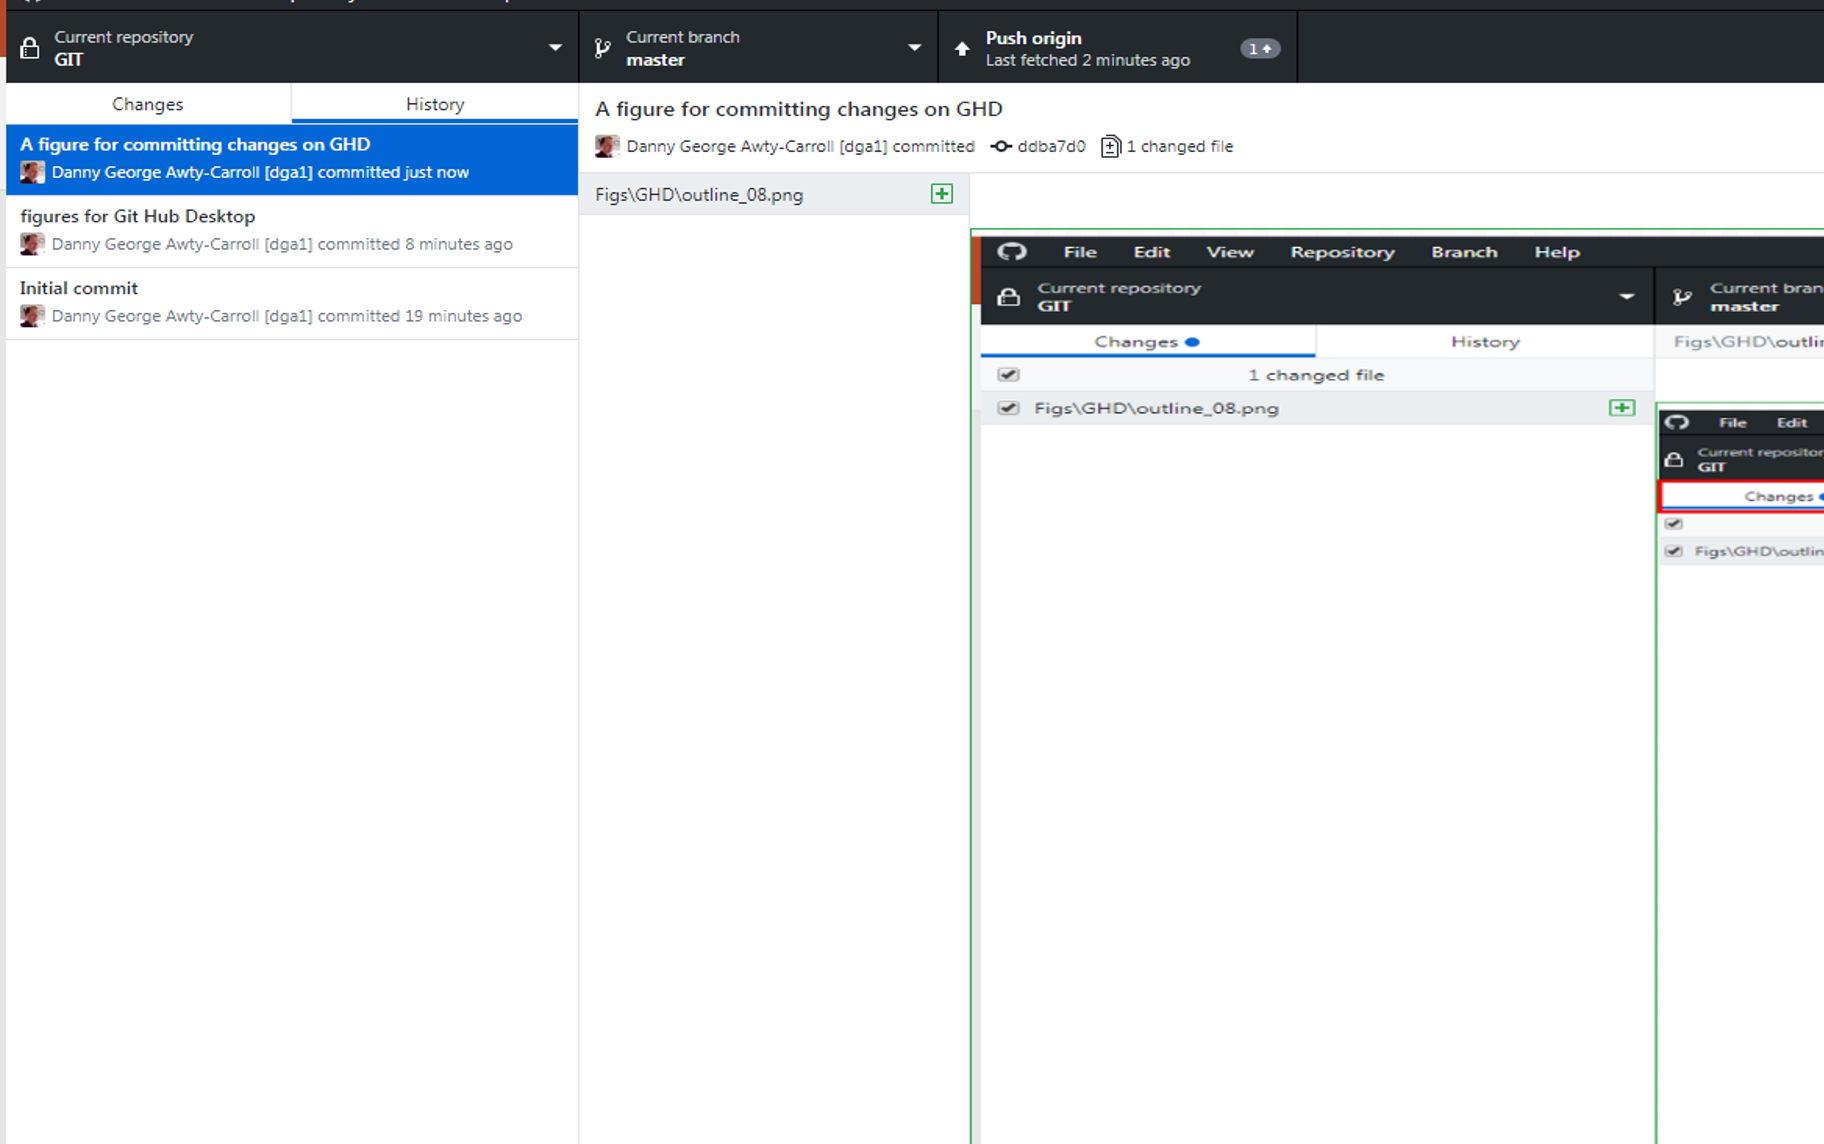
\includegraphics[width=12cm]{Figs/GHD/hist_00}
\end{frame}


\begin{frame}[fragile]{Using the repository}
\small Or look at how the files have changed from the records (same as \textit{git status})
\includegraphics[width=12cm]{Figs/GHD/outline_07}
\end{frame}


\begin{frame}[fragile]{Using the repository}
\small When there are changes you can make a new commit
\includegraphics[width=12cm]{Figs/GHD/outline_08}
\end{frame}

\begin{frame}[fragile]{Using the repository}
\small An example of some small changes to this presentation
\includegraphics[width=12cm]{Figs/GHD/outline_10}
\end{frame}

\section{Questions \& Demo}

{%
\setbeamertemplate{frame footer}{(xkcd)}
{\setbeamercolor{palette primary}{fg=gray, bg=gray}
\begin{frame}[standout]
\includegraphics[width=11cm]{Figs/xkcd_end}
\end{frame}
}


%\begin{frame}[fragile]{Backup slides}
% Sometimes, it is useful to add slides at the end of your presentation to
% refer to during audience questions.

% The best way to do this is to include the \verb|appendixnumberbeamer|
% package in your preamble and call \verb|\appendix| before your backup slides.

% \themename will automatically turn off slide numbering and progress bars for
% slides in the appendix.
%\end{frame}


\end{document}

